\documentclass[12pt,a4paper]{report}

% ============================================================
% University of Zambia - Department of Computing and Informatics
% Final Year Project Report - Academic Year 2026
% VeriScreen and the HELSB officer portal
% ============================================================

\usepackage[a4paper,margin=1in,left=1.25in]{geometry}
\usepackage{newtxtext,newtxmath}
\usepackage{setspace}
\usepackage{graphicx}
\usepackage{tikz}
\usetikzlibrary{arrows.meta,positioning,shapes.geometric}
\graphicspath{{figures/}}
\usepackage{booktabs}
\usepackage{longtable}
\usepackage{array}
\usepackage{float}
\usepackage{enumitem}
\usepackage{url}
\usepackage[hidelinks]{hyperref}
\usepackage{caption}
\usepackage{fancyhdr}
\usepackage{titlesec}
\usepackage{tocloft}

\onehalfspacing
\setlength{\parindent}{0.5in}
\setlength{\parskip}{0pt}

\pagestyle{fancy}
\fancyhf{}
\fancyhead[L]{Final Year Project Report}
\fancyhead[R]{2026}
\fancyfoot[C]{\thepage}

\titleformat{\chapter}[display]
  {\normalfont\bfseries\centering}
  {\chaptername\ \thechapter}
  {0.5em}
  {\Large}

\begin{document}

% ============================================================
% FRONT MATTER
% ============================================================

\begin{titlepage}
\centering
\vspace*{1cm}

{\Large\bfseries THE UNIVERSITY OF ZAMBIA\par}
\vspace{0.4cm}
{\large\bfseries SCHOOL OF NATURAL AND APPLIED SCIENCES\par}
\vspace{0.4cm}
{\large\bfseries DEPARTMENT OF COMPUTING AND INFORMATICS\par}

\vfill

{\Large\bfseries FINAL YEAR PROJECT REPORT\par}
\vspace{0.5cm}
{\large\bfseries ACADEMIC YEAR 2026\par}

\vfill

{\LARGE\bfseries VeriScreen: A Web-Based System for Academic Document Verification and HELSB Loan Screening\par}

\vfill

A Final Year Project Report Submitted to the\\
Department of Computing and Informatics\\
in partial fulfilment of the requirements for the award of\\[0.2cm]
{\bfseries the Bachelor's degree in the Department of Computing and Informatics}

\vfill

{\bfseries Students:}\\[0.3cm]
Samuel Chibinji Mwanza \quad Computer Number 2021465934\\
Nosiku Mukuka \quad Computer Number 2022030346\\[0.5cm]
{\bfseries Supervisor:} Mrs.\ Monde Monica Kalumbilo Kabemba\\[0.3cm]
{\bfseries Date of Submission:} 23rd October 2026

\vfill
\end{titlepage}

\chapter*{DECLARATION}
\addcontentsline{toc}{chapter}{Declaration}

We declare that this final year project report is our own work and has been prepared in accordance with the academic requirements of the University of Zambia. All sources of information, ideas, data, software, images, and other material that are not our own have been appropriately acknowledged and referenced.

This project was undertaken as a group. The report describes the system produced by the group. Where a component was completed jointly, it is described as joint work. We have not presented unpublished work of any other person as our own.

\vspace{1cm}
\noindent\textbf{Student Name:} Samuel Chibinji Mwanza

\vspace{0.5cm}
\noindent\textbf{Computer Number:} 2021465934

\vspace{0.5cm}
\noindent\textbf{Signature:} \hrulefill

\vspace{0.5cm}
\noindent\textbf{Date:} \hrulefill

\vspace{1cm}
\noindent\textbf{Student Name:} Nosiku Mukuka

\vspace{0.5cm}
\noindent\textbf{Computer Number:} 2022030346

\vspace{0.5cm}
\noindent\textbf{Signature:} \hrulefill

\vspace{0.5cm}
\noindent\textbf{Date:} \hrulefill

\clearpage

\chapter*{APPROVAL}
\addcontentsline{toc}{chapter}{Approval}

This final year project report has been submitted for examination with the approval of the project supervisor.

\vspace{1cm}
\noindent\textbf{Supervisor Name:} Mrs.\ Monde Monica Kalumbilo Kabemba

\vspace{0.5cm}
\noindent\textbf{Signature:} \hrulefill

\vspace{0.5cm}
\noindent\textbf{Date:} \hrulefill

\vspace{1cm}
\noindent\textbf{Departmental/Examiner Approval (if applicable):} \hrulefill

\clearpage

\chapter*{ABSTRACT}
\addcontentsline{toc}{chapter}{Abstract}

Students who apply for support from the Higher Education Loans and Scholarships Board must present academic documents that a lender can trust, and the lender must be able to explain why an application is approved or refused. Paper statements and informal screenshots are difficult to check, and a status such as ``approved'' does not tell the student which university record produced the decision. This project designed and implemented VeriScreen, a student web portal, together with a separate HELSB officer portal. The student portal shows registration, fees, examinations, and results taken from a simulated university record, and it issues those records as PDF documents sealed with a QR verification code. A phone that scans the code opens a page stating whether the document was issued. When a student applies for a loan, an officer moves the application through submission, portal confirmation, payment, screening, contract, and disbursement. At screening, the system reads the latest fee balance, registration, examination standing, and published grades, and it writes a plain-language result such as ``Not eligible: outstanding fee balance of K500.00'' or ``Approved: good academic standing, fees cleared, registration confirmed.'' The student dashboard shows the same stage and sentence. The completed system runs locally as two React applications and two Node.js services over MySQL. Testing with four seeded students confirmed login, PDF content, QR verification, live tracker updates, and the screening sentences.

\noindent\textbf{Keywords:} academic document verification; QR codes; student information systems; HELSB; loan screening

\clearpage

\chapter*{ACKNOWLEDGEMENTS}
\addcontentsline{toc}{chapter}{Acknowledgements}

We thank the Department of Computing and Informatics for the opportunity to undertake this final year project, and our supervisor for guidance during the work. We also acknowledge the Higher Education Loans and Scholarships Board as the institutional setting that motivated a clearer link between university records and loan decisions. The academic figures used in the demonstration come from a simulated university record prepared for this project. They are not a copy of a live University of Zambia production database.

\clearpage

\tableofcontents
\clearpage

\listoffigures
\clearpage

\listoftables
\clearpage

\chapter*{LIST OF ABBREVIATIONS AND ACRONYMS}
\addcontentsline{toc}{chapter}{List of Abbreviations and Acronyms}

\begin{longtable}{p{0.28\textwidth}p{0.62\textwidth}}
\textbf{Abbreviation} & \textbf{Meaning}\\
API & Application Programming Interface\\
CRUD & Create, read, update, and delete\\
GPA & Grade point average\\
HELSB & Higher Education Loans and Scholarships Board\\
HTTP & Hypertext Transfer Protocol\\
JWT & JSON Web Token\\
NRC & National Registration Card\\
PDF & Portable Document Format\\
QR & Quick Response code\\
REST & Representational State Transfer\\
SIS & Student Information System\\
SQL & Structured Query Language\\
UI & User Interface\\
UNZA & University of Zambia\\
\end{longtable}

\clearpage

\chapter*{NOTE ON GROUP PROJECTS}
\addcontentsline{toc}{chapter}{Note on Group Projects}

This report is the group account of one shared system. Samuel Chibinji Mwanza (2021465934) and Nosiku Mukuka (2022030346) worked on VeriScreen and the HELSB officer portal as a single product. The student portal, the officer portal, the document service, and the screening rules are parts of that product. Appendix~A records the joint contribution and leaves a precise percentage split to be confirmed with the supervisor before the report is bound. Neither student claims a module that the repository presents as separate personal property of the other.

\clearpage

\chapter{Introduction}

\section{Background and Context}
Zambian undergraduate students routinely need official evidence of registration, fees, and results. The same evidence is required when a student seeks a loan or scholarship from the Higher Education Loans and Scholarships Board. In current practice, a student may download or photograph a portal page and send that image to a sponsor. The recipient cannot easily tell whether the image still matches the university record, whether a balance has changed, or which rule produced a later loan decision.

VeriScreen addresses that gap as a student-facing web system. It presents the academic record, issues it as a PDF, and attaches a verification code that a third party can scan. Beside it, a separate officer portal lets HELSB staff move an application through a visible pipeline and record an explainable screening result. The two sites do not share a login. A student cannot open the officer screens, and an officer cannot sign in to the student portal with an officer account.

The demonstration uses a simulated University of Zambia record for a small set of students. The figures on each document are read from that record. They are not typed into the PDF by hand and they are not copied from a screenshot.

\section{Problem Statement}
Students lack a single place in which an academic document can be issued from the university record and later checked by someone who was not present when it was downloaded. HELSB officers, in turn, can be shown a loan percentage or a status word without a sentence that ties the decision to fees, registration, examinations, and grades. The project therefore addresses two related problems: proof that a document was issued, and an explanation of why screening reached its result.

\section{Project Aim}
The aim of this project is to build a working web system that issues verifiable academic documents from a simulated university record and explains HELSB screening decisions in plain language.

\section{Project Objectives}
\begin{enumerate}
    \item Provide a student portal on which a student can sign in and view registration, fees, examinations, and results held for that student.
    \item Generate PDF documents whose content is taken from those records, including a fee statement, academic results, and a confirmation of registration.
    \item Allow a phone to scan a QR code on an issued document and display whether VeriScreen issued that document.
    \item Provide a separate HELSB officer portal that can receive an application and move it through a defined pipeline visible to the student.
    \item When screening runs, compute a plain-language result from the fee balance, registration, examination standing, and academic results, and show that sentence to both the officer and the student.
\end{enumerate}

\section{Research Questions (where applicable)}
The project is a design-and-build project rather than a statistical study. The questions that guided the build were the following.
\begin{enumerate}
    \item Can an issued PDF be checked later without trusting a screenshot?
    \item Can a loan decision be stated as a sentence that a student can match to a university record?
    \item Can the student view and the officer view stay consistent while the application moves?
\end{enumerate}

\section{Scope of the Project}
\subsection{In Scope}
The completed project includes the student web portal, the HELSB officer web portal, the student API, the officer API, MySQL storage for both, PDF generation, QR verification, the application tracker, and the screening explanation. The student portal is laid out for a desktop window and for a phone-width window. An Expo client that calls the same student API is included in the repository. Seeded demonstration students and officers are included so that the workflow can be exercised without a live university or HELSB connection.

\subsection{Out of Scope}
The project does not replace the University of Zambia student information system and does not connect to a production HELSB database. It does not disburse real money, sign a legally binding loan contract, or perform biometric identity checks. The illustrations in this report are screenshots of the web portals, including the student portal at phone width, together with diagrams of the design. Forgotten-password and self-registration flows were removed from the student sign-in page so that access stays limited to issued accounts.

\section{Significance of the Project}
Students gain a document that can be shown to a sponsor and checked afterwards. Officers gain a screening result they can read aloud and defend from the record. The department gains a concrete example of a multi-application information system in which authority is split: the university record supplies facts, VeriScreen issues documents, and HELSB staff control the loan pipeline.

\section{Limitations}
The academic data are simulated. Screening uses rules chosen for this project, including a latest-balance test and a grade-point threshold, and those rules are not a published HELSB regulation. QR verification confirms that VeriScreen issued the code. It does not detect a visually edited photocopy if the code itself is left unchanged, and it does not re-check the PDF bytes. Phone scanning requires the phone and the computer to be on a reachable network, and a host firewall can block the verification port. The supervisor's name is not printed on the title page because it was not available when this report was generated.

\section{Organisation of the Report}
Chapter~2 reviews document verification, loan screening, and the related technical ideas. Chapter~3 describes how the system was built and how it was evaluated. Chapter~4 records the requirements and the design. Chapter~5 describes the implementation. Chapter~6 reports the tests. Chapter~7 discusses what the results mean. Chapter~8 concludes and recommends further work. The appendices contain the group contribution statement and operating notes.

\chapter{Literature Review}

\section{Introduction}
This chapter sets out the ideas required to understand the system: official academic records, the role of a loans board, machine-checkable documents, and the separation between a student application and an officer decision.

\section{Key Concepts and Theories}
An academic record is authoritative only while it remains tied to the institution that holds it. A downloaded file becomes a copy. A useful verification scheme therefore stores an identifier at issue time and resolves that identifier later against the issuing system. A QR code is a two-dimensional barcode that can carry a short web address [2]. The phone does not need a special application if the address opens in a browser.

Loan screening is a decision procedure. A percentage or a colour can summarise the outcome, but it does not state the premise. An explainable decision names the fact that failed or the facts that passed. In this project those facts are the outstanding fee balance, confirmation of registration, examination eligibility, and academic standing derived from published grades.

The architecture follows a REST style: clients call named HTTP resources, and each service keeps its own data [4]. Authentication uses a JSON Web Token [3]. The token shows that a sign-in succeeded. It does not by itself prove that a document is genuine. Document trust is handled by the verification identifier, not by the student's session.

\section{Existing Systems / Related Work}
University portals commonly let a student view fees, registration, and results. Those pages are useful to the student and weak as evidence for a third party, because a screenshot can be cropped or edited. A separate loans board then receives whatever the student chooses to send.

The Higher Education Loans and Scholarships Board is the Zambian body charged with administering higher-education loans and scholarships [1]. Its officers need student identity, programme, registration, fee clearance, and academic progress. Those facts originate at the university. A system that only stores a loan percentage breaks that link.

General document systems such as digitally signed PDFs can prove that bytes were not changed after signing. That approach needs certificate management. This project uses a lighter check that is enough for a demonstration: the QR code points at the issuing server, and the server reports whether that code was issued, to whom, and as which document type.

\section{Comparative Analysis}
Table~\ref{tab:compare} compares three ways a sponsor might receive an academic document.

\begin{table}[H]
\centering
\caption{Comparison of ways to present an academic document}
\label{tab:compare}
\begin{tabular}{p{0.22\textwidth}p{0.22\textwidth}p{0.22\textwidth}p{0.22\textwidth}}
\toprule
Criterion & Screenshot & Signed PDF only & VeriScreen QR\\
\midrule
Readable by a person & Yes & Yes & Yes\\
Tied to a student record & No & Only if generated from it & Yes, at issue time\\
Checkable on a phone & No & Only with extra tools & Yes, by scanning\\
Explains a later loan decision & No & No & Yes, in the officer and student views\\
\bottomrule
\end{tabular}
\end{table}

A signed PDF is stronger against byte-level tampering. VeriScreen is stronger for the demonstration constraint that a phone camera and a browser must be enough, and that the loan decision must be readable as a sentence.

\section{Research / Knowledge Gap}
Existing student portals and loan files do not, in the setting studied here, give a third party a simple check of an issued document and give the student a sentence that cites the fee balance or the academic standing. The gap is not the absence of databases. It is the absence of a checkable document and an explainable screening step between the university record and the loans board.

\section{Conceptual or Theoretical Framework (where applicable)}
The project uses a three-role framework.
\begin{enumerate}
    \item The university record is the source of academic facts.
    \item VeriScreen is the issuer of documents and the student's view of the loan pipeline.
    \item The HELSB officer portal is the place where staff advance that pipeline and where screening is run.
\end{enumerate}
A fact may be copied into VeriScreen so that a document can be generated when the original system is not online. The screening sentence is computed from the copy held for the student at the moment screening runs.

\section{Chapter Summary}
Screenshots are poor evidence. A QR address checked against the issuer is a practical alternative for a phone. Loan screening is more useful when it states the record that produced the result. The project applies those ideas by separating the student portal from the officer portal and by generating both the document and the screening sentence from the same student record.

\chapter{Methodology}

\section{Introduction}
The project was conducted as a design-and-build exercise. The method was to fix the requirements from the student and officer workflows, implement them as running web applications, and evaluate them against those workflows rather than against a survey sample.

\section{Research / Development Approach}
Development followed short increments. Each increment had a visible result: student sign-in, records, PDF layout, phone verification, the officer tracker, and then the screening sentence. A change was kept when it could be demonstrated in the browser or by calling the API. This is closer to an incremental delivery approach than to a single waterfall handover, although the requirements were written down before each increment so that the scope did not drift into unrelated features.

An earlier design in the repository used Java services and PostgreSQL. The completed local system was moved to Node.js and MySQL so that it could run with a widely available database and so that the student site and the officer site could be started without a Java runtime. The behaviour required by the objectives was preserved: issued documents, separated officer access, and a status the student can see.

\section{Requirements / Data Collection}
Requirements were taken from the workflows a student and an officer must complete, not from a field questionnaire. The academic figures were seeded from a simulated university record for four primary students: Samuel Chibinji Mwanza, Nosiku Mukuka, Grace Banda, and Peter Zulu. Fee amounts, registration flags, examination status, and grades are stored in MySQL and read at document generation and at screening. No live student was interviewed, and no production university extract was used.

\section{System Architecture / Research Workflow}
The running system has four processes.

\begin{table}[H]
\centering
\caption{Running parts of the completed system}
\label{tab:processes}
\begin{tabular}{p{0.28\textwidth}p{0.18\textwidth}p{0.40\textwidth}}
\toprule
Part & Address & Responsibility\\
\midrule
Student web portal & localhost:5173 & Sign-in, records, documents, tracker\\
Student API & port 8081 & Identity, PDFs, verification, student copy of the pipeline\\
HELSB web portal & localhost:5174 & Universities, schools, applications, screening\\
HELSB API & port 8083 & Officer identity, pipeline, call to screening\\
\bottomrule
\end{tabular}
\end{table}

The student API stores students, fees, registrations, examinations, results, issued documents, and the student's copy of the HELSB application in \texttt{veriscreen\_db}. The officer API stores officers and applications in \texttt{helsb\_db}. When an officer advances an application, the officer API notifies the student API with a shared internal key. When the next stage is screening, the officer API asks the student API to explain the record before the stage is saved.

\section{Tools and Technologies}
Table~\ref{tab:tools} lists the tools used in the completed build.

\begin{table}[H]
\centering
\caption{Tools and technologies}
\label{tab:tools}
\begin{tabular}{p{0.32\textwidth}p{0.55\textwidth}}
\toprule
Tool & Use in the project\\
\midrule
React and TypeScript & Student portal and officer portal\\
Vite & Development server and proxy to each API\\
Node.js and Express & Both HTTP APIs\\
MySQL & \texttt{veriscreen\_db} and \texttt{helsb\_db}\\
PDFKit & Fee, results, confirmation, and related PDFs\\
QR code library & Address embedded in each PDF\\
JSON Web Tokens & Student and officer sessions\\
bcrypt & Password hashes\\
\bottomrule
\end{tabular}
\end{table}

PostgreSQL remains supported when a deployment URL is supplied, which allows the same API code to run against a hosted PostgreSQL database. The local demonstration uses MySQL.

\section{Ethical and Legal Considerations}
The students in the database are demonstration identities created for the project. National registration numbers in that seed are fictional. The system does not collect live biometric data and does not send documents to an external loans board. Officer and student passwords in the seed are development passwords and are not suitable for a public deployment. The verification page reveals the student name, computer number, and document type for a code that was issued. It does not reveal grades or fee amounts. That is intentional: a person who scanned a document the student chose to share can confirm the issue, but the code alone is not a full academic transcript.

\section{Evaluation Method}
Success was defined as the observable behaviour in the objectives. A test passed when the screen or the API response matched the record. Representative cases used the seeded students because their fee balances and grades are known in advance. Samuel has a latest outstanding balance of K500.00. Nosiku has cleared fees, confirmed registration, and published grades. Grace Banda and Peter Zulu have outstanding balances. No claim is made about usability scores, because a formal user study was not conducted.

\section{Chapter Summary}
The system was built in increments and judged by whether a student can obtain a document, a phone can check it, an officer can move the pipeline, and screening can explain itself from the stored record.

\chapter{System Analysis and Design}

\section{Introduction}
This chapter records who uses the system, what it must do, and how the main parts are arranged.

\section{Stakeholder and User Analysis}
\begin{table}[H]
\centering
\caption{Stakeholders and what they need}
\label{tab:stakeholders}
\begin{tabular}{p{0.28\textwidth}p{0.58\textwidth}}
\toprule
Stakeholder & Need\\
\midrule
Student & See the academic record, download a PDF, and follow the loan pipeline\\
Sponsor or verifier & Scan a code and see whether the document was issued\\
HELSB officer & Open an application, advance it, and read the screening sentence\\
University (simulated) & Remain the origin of fees, registration, examinations, and grades\\
Department & A demonstrable final-year system with a written account\\
\bottomrule
\end{tabular}
\end{table}

\section{Functional Requirements}
\begin{enumerate}
    \item The student signs in with a computer number and password.
    \item The student sees a dashboard with a personal welcome, the HELSB tracker, recent documents, and recent activity.
    \item The student can open registration, fee history, and results drawn from the stored record.
    \item The student can preview and download an issued PDF.
    \item A verification address on the PDF returns a page that states whether the code was issued and names the student and document type.
    \item The student can submit an application to HELSB. Seeded applications already exist for the demonstration students.
    \item An officer signs in with an officer email and password on a separate site.
    \item The officer browses universities, schools, and applications.
    \item The officer advances the pipeline one stage at a time.
    \item Entering screening computes and stores a plain-language explanation.
    \item A result that begins ``Not eligible'' stops the pipeline at screening.
    \item An approved result allows the officer to continue to contract and disbursement.
    \item The student tracker updates to the same stage and shows the same sentence.
\end{enumerate}

\section{Non-Functional Requirements}
The student interface keeps the established VeriScreen colours: a dark green sidebar and gold accents. The officer interface is a separate layout so that the two organisations are not confused. Passwords are stored as hashes. Officer and student tokens are different secrets. The internal call from the officer API to the student API requires a shared key. Pages that a phone will open must be readable on a narrow screen. The local system must start without a Java runtime.

\section{Use Cases / User Stories}
The main stories are the following.
\begin{enumerate}
    \item As a student, I sign in so that I see only my record.
    \item As a student, I download a fee statement so that the figures match my stored payments and balance.
    \item As a verifier, I scan the QR code so that I see a clear verified or not-verified page.
    \item As an officer, I open a school and an application so that I can move the loan pipeline.
    \item As a student, I watch the dashboard so that I see the stage the officer has reached and, after screening, the reason.
\end{enumerate}

\section{System / Solution Architecture}
The browser never reads MySQL directly. The student portal calls the student API. The officer portal calls the officer API. Those APIs do not share tables. The only bridge is the internal HTTP call used for the tracker and for screening. This keeps an officer action from becoming a direct write into student tables by the officer process, and it keeps the sentence in one place: the student API computes it, and both databases store the text that was returned.

Screening applies the first matching rule in Table~\ref{tab:rules}.

\begin{table}[H]
\centering
\caption{Screening rules, applied in order}
\label{tab:rules}
\begin{tabular}{p{0.42\textwidth}p{0.48\textwidth}}
\toprule
Condition on the student record & Sentence\\
\midrule
No fee row & Not eligible: no fee record is available.\\
Latest outstanding balance greater than zero & Not eligible: outstanding fee balance of K\textit{amount}\\
Latest registration not confirmed & Not eligible: registration is not confirmed.\\
Latest examination blocked or not eligible & Not eligible: examinations are blocked.\\
No published results, a failing grade, or GPA below 2.00 & Not eligible: academic standing is below the required level.\\
Otherwise & Approved: good academic standing, fees cleared, registration confirmed.\\
\bottomrule
\end{tabular}
\end{table}

GPA uses the credit-weighted scale A and A+ = 4.0, A$-$ = 3.7, B+ = 3.3, B = 3.0, and so on down to F = 0.

\section{Database / Data Design (where applicable)}
\texttt{veriscreen\_db} holds students, registrations, fees, examinations, academic results, issued documents, notifications, and HELSB application rows including the pipeline stage and the screening explanation. \texttt{helsb\_db} holds officers, applications, and status history. An application row stores the student computer number, programme, school, document identifiers, pipeline stage, and the explanation text. The two databases can therefore disagree only if the internal notification fails. The officer action still saves the officer-side stage, and the error is written to the server log.

\section{Interface / Interaction Design (where applicable)}
The student home is a dashboard, not a dump of every table. Fees and results have their own pages. Documents open as PDFs in a preview and as downloads. The HELSB area shows the application and the screening sentence when one exists. The officer home is a list of universities, then schools, then applications. The application page shows the six pipeline steps and one button for the next step. After screening, the sentence is shown on that page in green when it starts with ``Approved'' and in red when it starts with ``Not eligible''. Settings offers a dark-mode switch and email notifications. Help sits above Settings, and sign-out asks for confirmation. On a narrow screen the sidebar becomes a menu. The QR code on each PDF carries the time the document was issued, and the verification page prints that time.

\section{Design illustrations}
The diagrams in this section describe the structure. The screenshots that follow were taken from the running system on 19 October 2026, signed in as Samuel Chibinji Mwanza on the student portal and as officer Mwaka Chanda on the HELSB portal.

\begin{figure}[H]
\centering
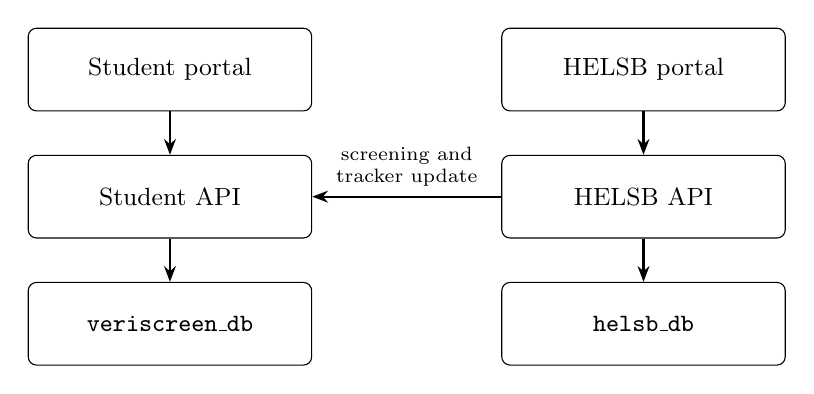
\begin{tikzpicture}[
  node distance=0.55cm and 1.5cm,
  box/.style={draw, rounded corners=3pt, align=center, minimum width=3.6cm, minimum height=1.05cm, font=\small, fill=white},
  arr/.style={-{Stealth[length=2mm]}, thick}
]
\node[box] (web) {Student portal};
\node[box, below=of web] (api) {Student API};
\node[box, below=of api] (db1) {\texttt{veriscreen\_db}};
\node[box, right=2.4cm of web] (oweb) {HELSB portal};
\node[box, below=of oweb] (oapi) {HELSB API};
\node[box, below=of oapi] (db2) {\texttt{helsb\_db}};
\draw[arr] (web) -- (api);
\draw[arr] (api) -- (db1);
\draw[arr] (oweb) -- (oapi);
\draw[arr] (oapi) -- (db2);
\draw[arr] (oapi.west) -- node[midway, above, font=\scriptsize, align=center] {screening and\\tracker update} (api.east);
\end{tikzpicture}
\caption{Separation of the student portal and the HELSB officer portal}
\label{fig:architecture}
\end{figure}

\begin{figure}[H]
\centering
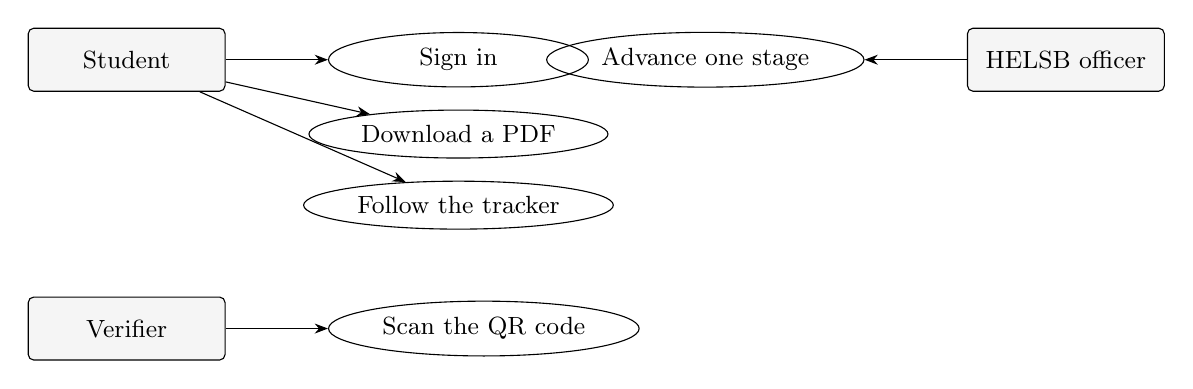
\begin{tikzpicture}[
  node distance=0.28cm and 1.3cm,
  person/.style={draw, rounded corners=2pt, align=center, font=\small, minimum width=2.5cm, minimum height=0.8cm, fill=gray!8},
  case/.style={draw, ellipse, align=center, font=\small, inner sep=3pt, minimum width=3.3cm}
]
\node[person] (student) {Student};
\node[case, right=of student] (sign) {Sign in};
\node[case, below=of sign] (pdf) {Download a PDF};
\node[case, below=of pdf] (watch) {Follow the tracker};
\node[person, right=4.8cm of sign] (officer) {HELSB officer};
\node[case, left=of officer] (advance) {Advance one stage};
\node[person, below=2.6cm of student] (phone) {Verifier};
\node[case, right=of phone] (scan) {Scan the QR code};
\draw[-{Stealth}] (student) -- (sign);
\draw[-{Stealth}] (student) -- (pdf);
\draw[-{Stealth}] (student) -- (watch);
\draw[-{Stealth}] (officer) -- (advance);
\draw[-{Stealth}] (phone) -- (scan);
\end{tikzpicture}
\caption{Principal use cases}
\label{fig:usecases}
\end{figure}

\begin{figure}[H]
\centering
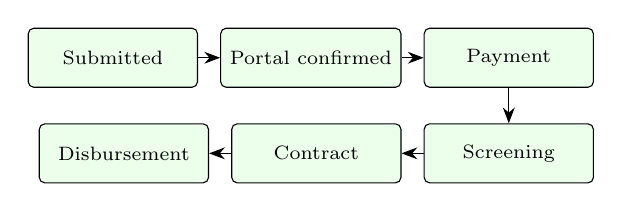
\begin{tikzpicture}[
  stage/.style={draw, rounded corners=2pt, align=center, font=\scriptsize, minimum width=2.15cm, minimum height=0.75cm, fill=green!8},
  arr/.style={-{Stealth[length=2mm]}}
]
\node[stage] (s1) {Submitted};
\node[stage, right=0.28cm of s1] (s2) {Portal confirmed};
\node[stage, right=0.28cm of s2] (s3) {Payment};
\node[stage, below=0.45cm of s3] (s4) {Screening};
\node[stage, left=0.28cm of s4] (s5) {Contract};
\node[stage, left=0.28cm of s5] (s6) {Disbursement};
\draw[arr] (s1) -- (s2);
\draw[arr] (s2) -- (s3);
\draw[arr] (s3) -- (s4);
\draw[arr] (s4) -- (s5);
\draw[arr] (s5) -- (s6);
\end{tikzpicture}
\caption{HELSB pipeline. A result that begins ``Not eligible'' stops at screening.}
\label{fig:pipeline}
\end{figure}

\begin{figure}[H]
\centering
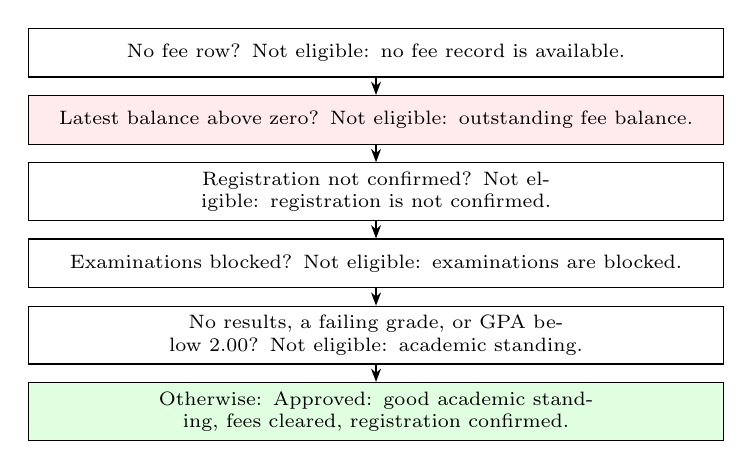
\begin{tikzpicture}[
  node distance=0.22cm,
  rule/.style={draw, align=center, font=\scriptsize, text width=8.6cm, minimum height=0.62cm, fill=white},
  stop/.style={draw, align=center, font=\scriptsize, text width=8.6cm, minimum height=0.62cm, fill=red!8},
  pass/.style={draw, align=center, font=\scriptsize, text width=8.6cm, minimum height=0.62cm, fill=green!12}
]
\node[rule] (a) {No fee row? Not eligible: no fee record is available.};
\node[stop, below=of a] (b) {Latest balance above zero? Not eligible: outstanding fee balance.};
\node[rule, below=of b] (c) {Registration not confirmed? Not eligible: registration is not confirmed.};
\node[rule, below=of c] (d) {Examinations blocked? Not eligible: examinations are blocked.};
\node[rule, below=of d] (e) {No results, a failing grade, or GPA below 2.00? Not eligible: academic standing.};
\node[pass, below=of e] (f) {Otherwise: Approved: good academic standing, fees cleared, registration confirmed.};
\draw[-{Stealth}] (a) -- (b);
\draw[-{Stealth}] (b) -- (c);
\draw[-{Stealth}] (c) -- (d);
\draw[-{Stealth}] (d) -- (e);
\draw[-{Stealth}] (e) -- (f);
\end{tikzpicture}
\caption{Screening checks, applied from top to bottom. The first match is the sentence stored for the student and the officer.}
\label{fig:screening}
\end{figure}

\begin{figure}[H]
\centering
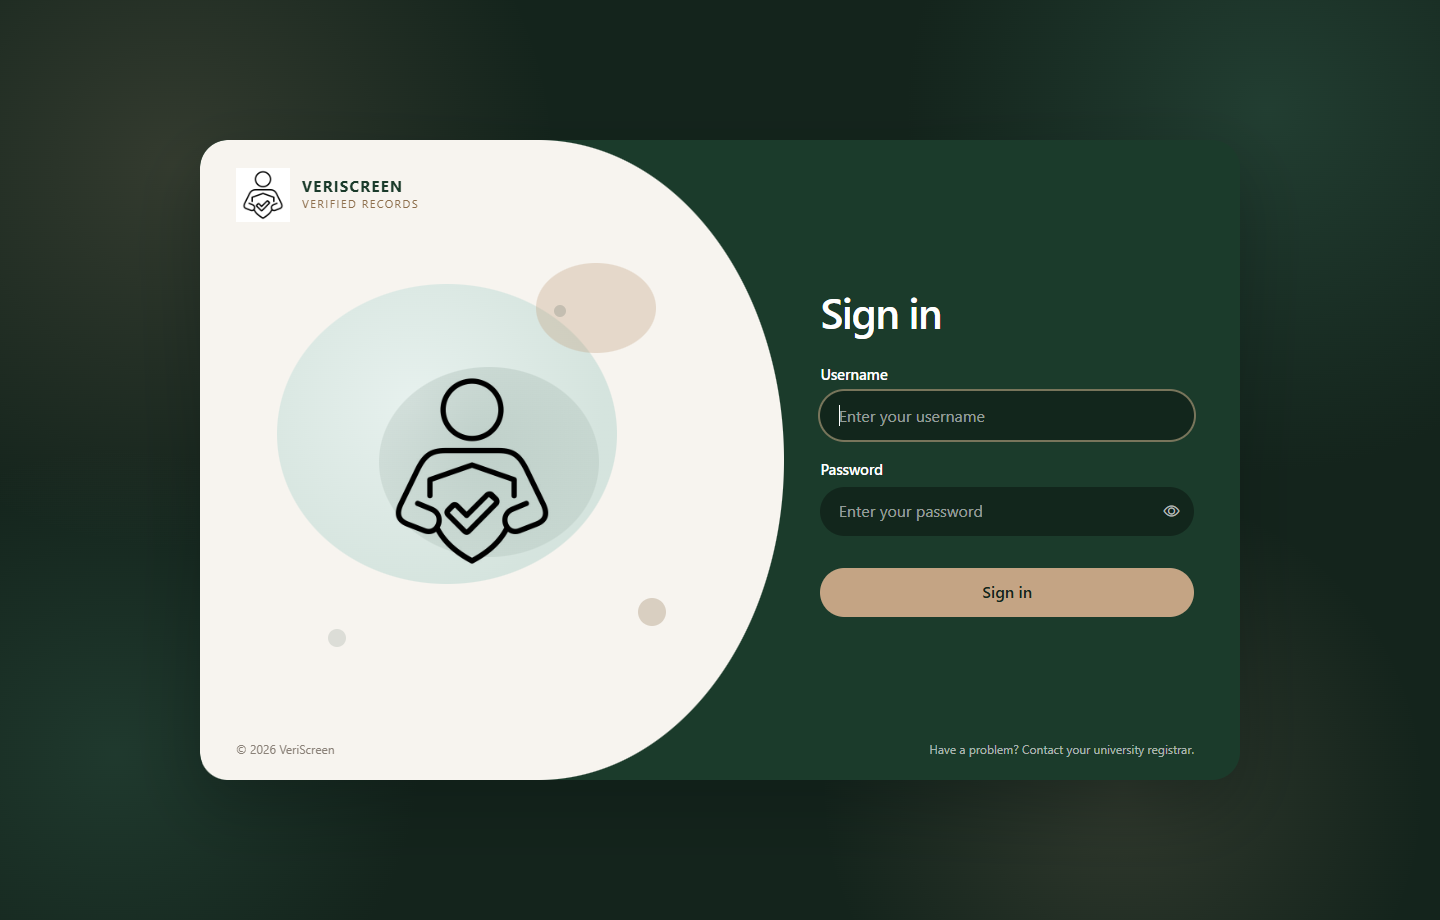
\includegraphics[width=0.92\textwidth]{vs-login-desktop.png}
\caption{VeriScreen sign-in at desktop width}
\label{fig:vs-login}
\end{figure}

\begin{figure}[H]
\centering
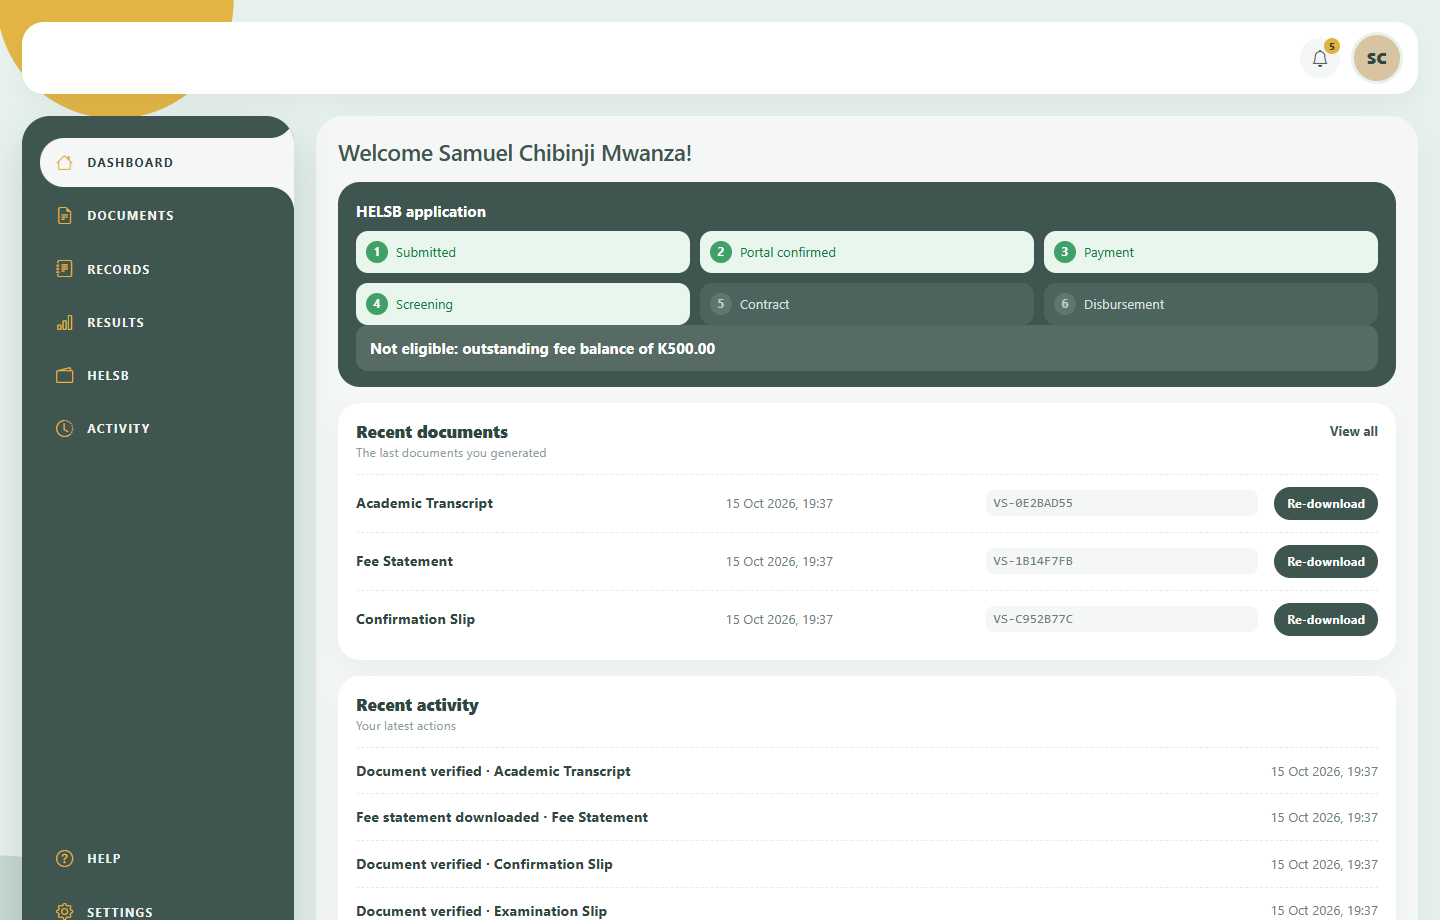
\includegraphics[width=\textwidth]{vs-dashboard-desktop.png}
\caption{Student dashboard for Samuel Chibinji Mwanza, with the tracker at screening}
\label{fig:vs-dashboard}
\end{figure}

\begin{figure}[H]
\centering
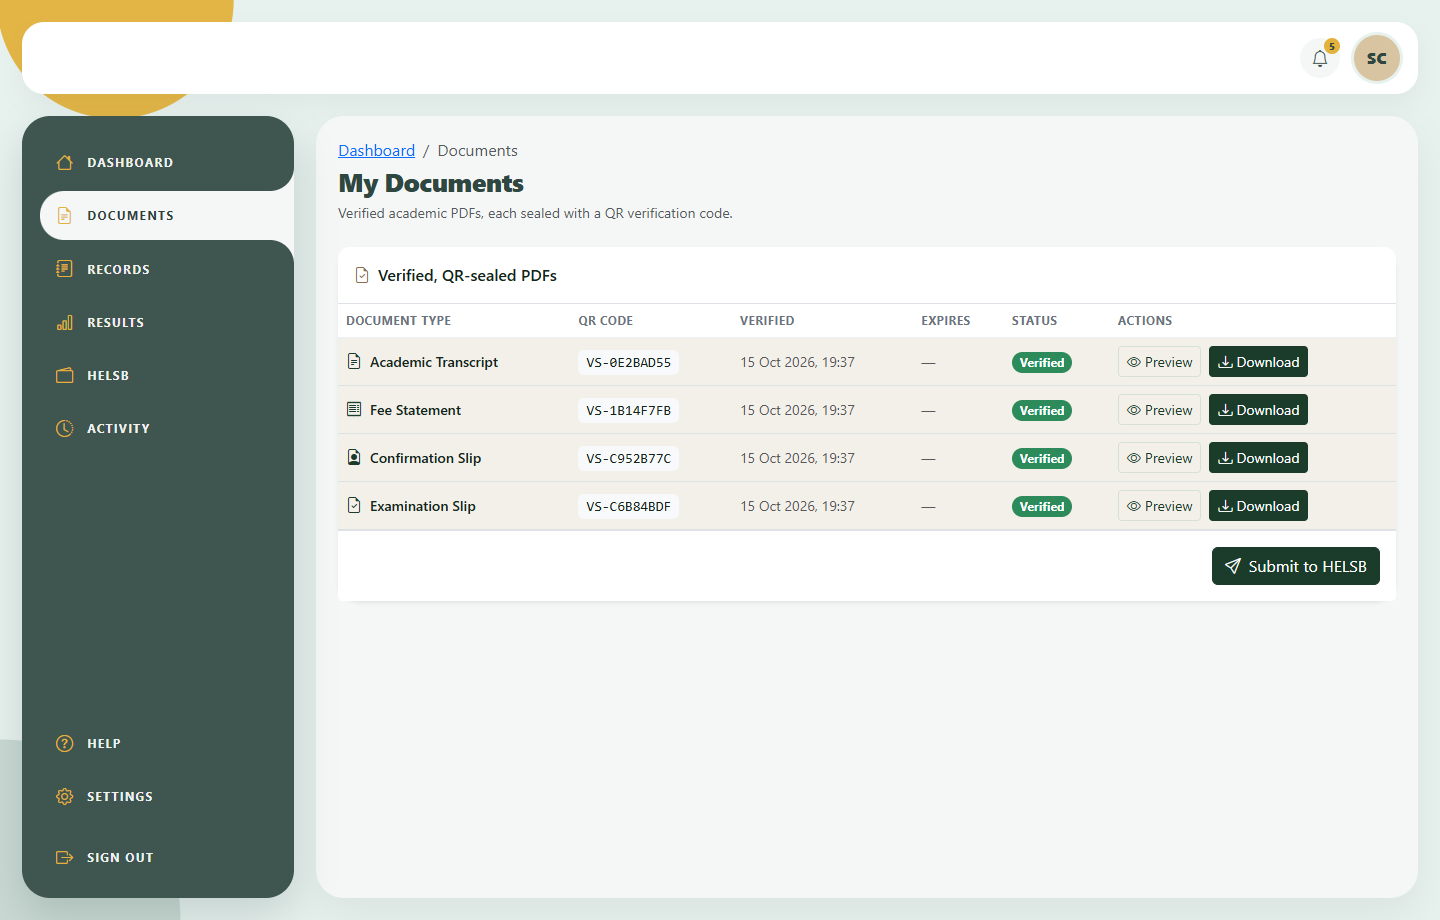
\includegraphics[width=\textwidth]{vs-documents-desktop.png}
\caption{Issued documents on the student portal}
\label{fig:vs-documents}
\end{figure}

\begin{figure}[H]
\centering
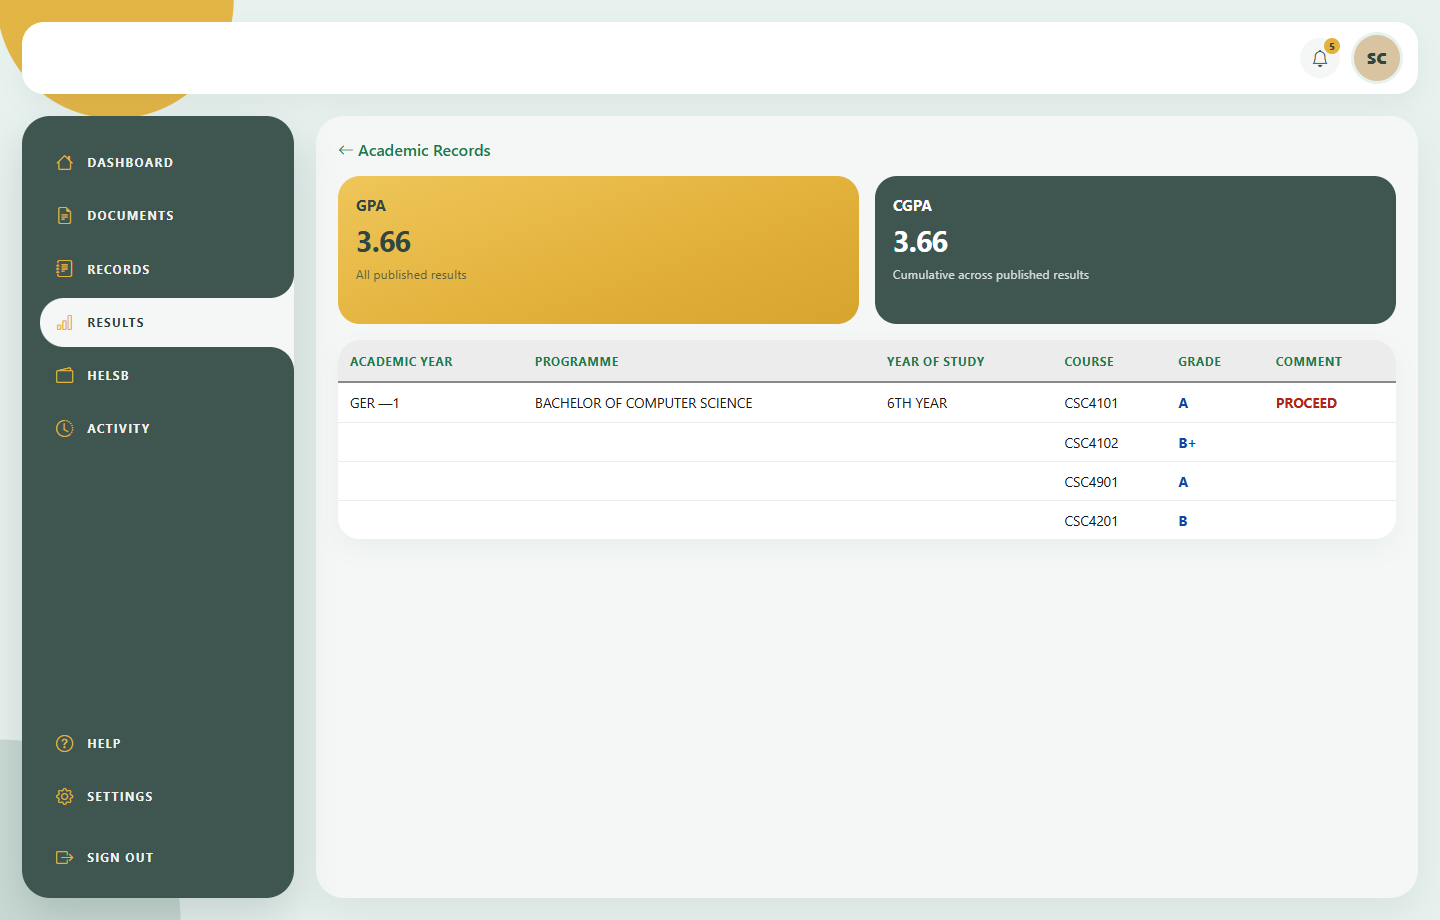
\includegraphics[width=\textwidth]{vs-results-desktop.png}
\caption{Published results for the signed-in student}
\label{fig:vs-results}
\end{figure}

\begin{figure}[H]
\centering
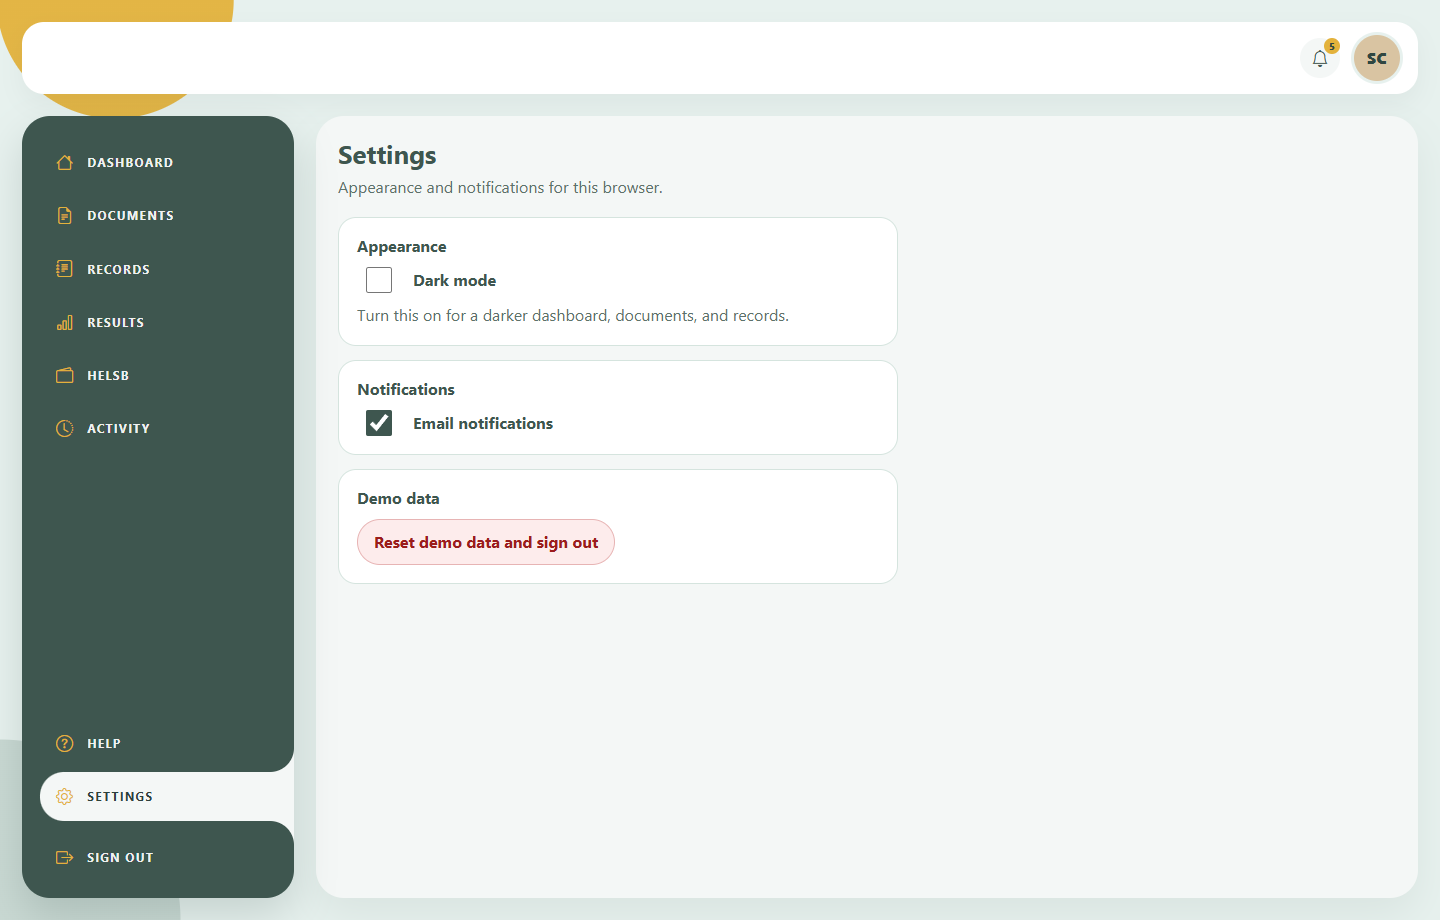
\includegraphics[width=\textwidth]{vs-settings-desktop.png}
\caption{Settings, with dark mode and email notifications. Help is the item above Settings in the sidebar.}
\label{fig:vs-settings}
\end{figure}

\begin{figure}[H]
\centering
\begin{minipage}[t]{0.46\textwidth}
\centering
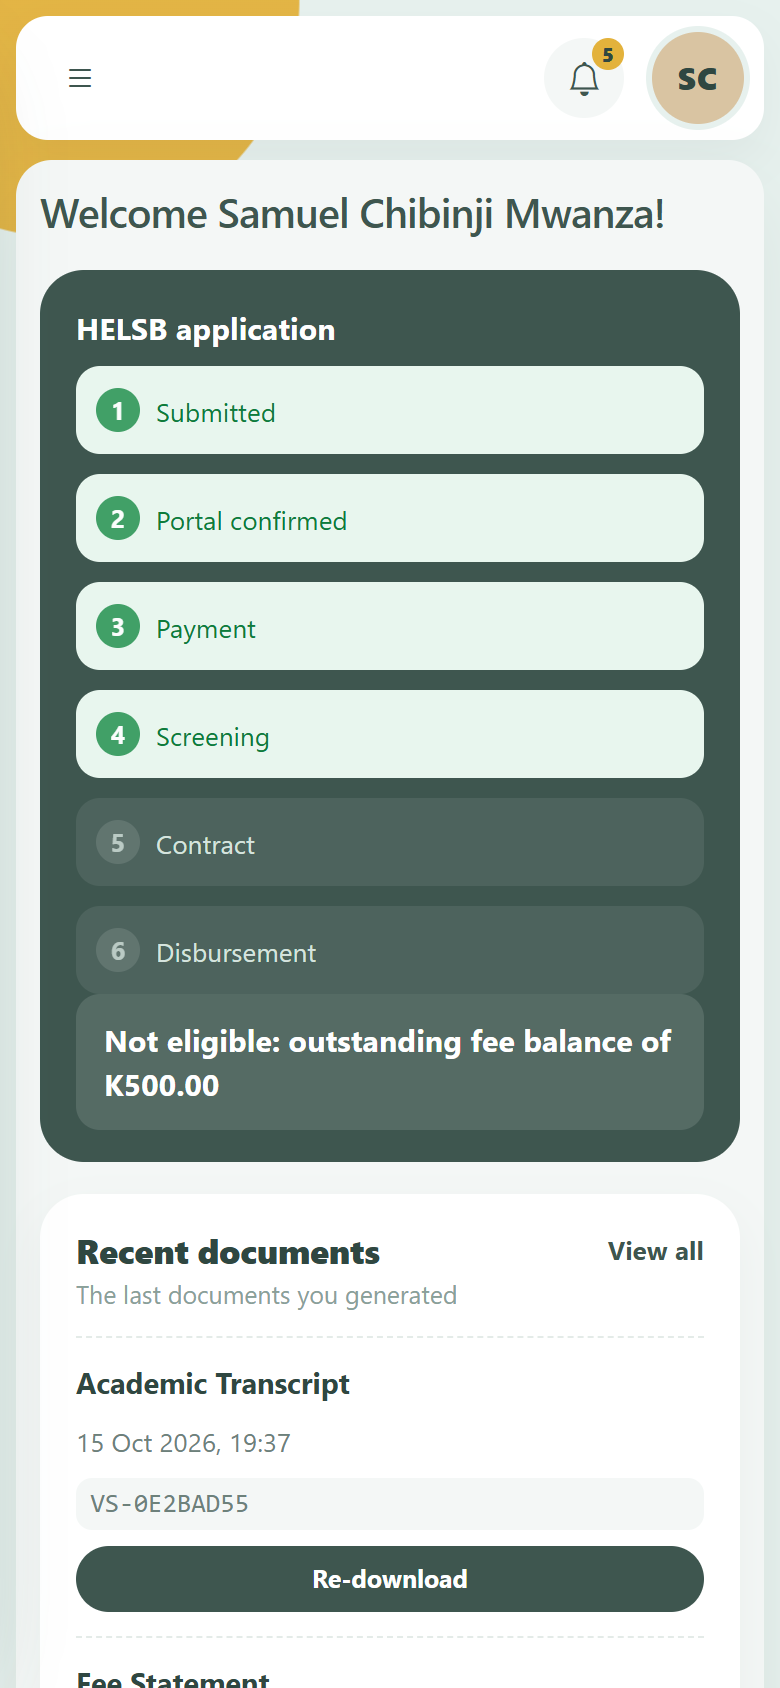
\includegraphics[width=\linewidth]{vs-dashboard-mobile.png}
\end{minipage}\hfill
\begin{minipage}[t]{0.46\textwidth}
\centering
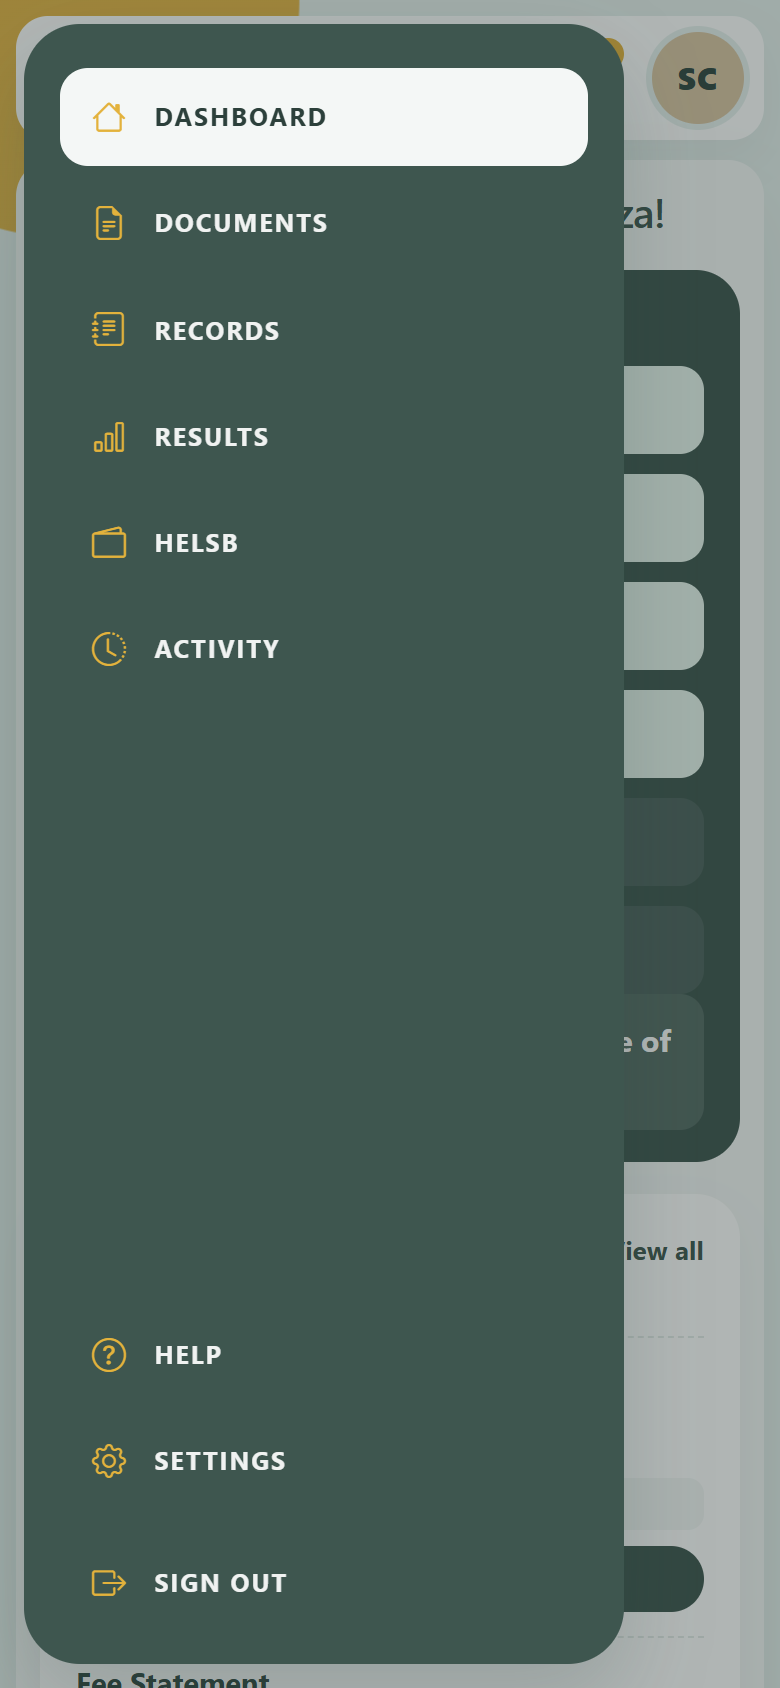
\includegraphics[width=\linewidth]{vs-menu-mobile.png}
\end{minipage}
\caption{VeriScreen at phone width: the dashboard, and the menu that replaces the sidebar}
\label{fig:vs-mobile}
\end{figure}

\begin{figure}[H]
\centering
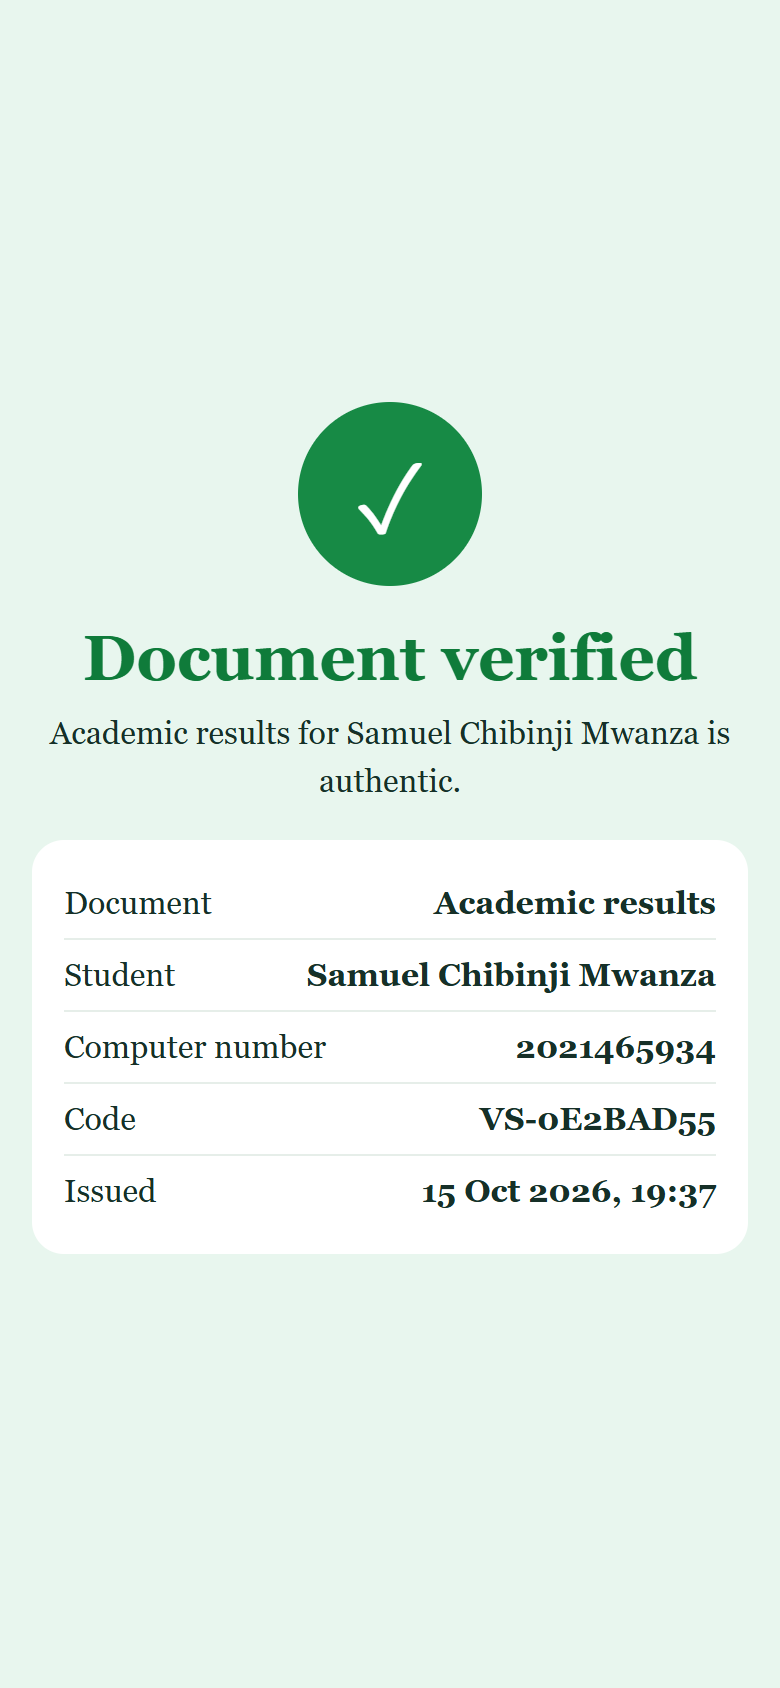
\includegraphics[width=0.42\textwidth]{vs-verify-mobile.png}
\caption{Page opened from a document QR code, including the issued time}
\label{fig:verify}
\end{figure}

\begin{figure}[H]
\centering
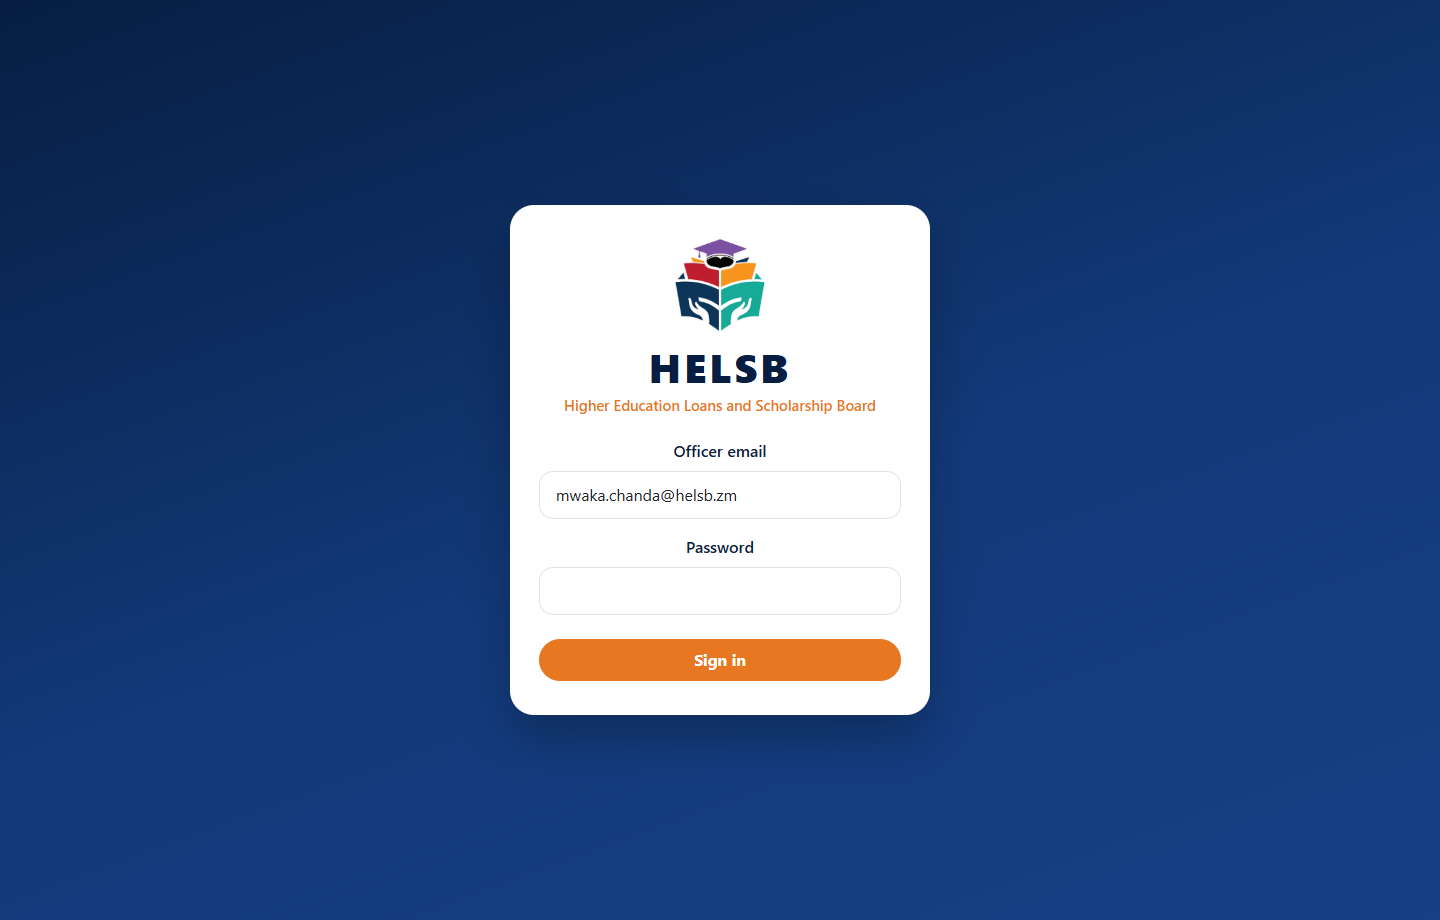
\includegraphics[width=0.72\textwidth]{helsb-login-desktop.png}
\caption{HELSB officer sign-in}
\label{fig:helsb-login}
\end{figure}

\begin{figure}[H]
\centering
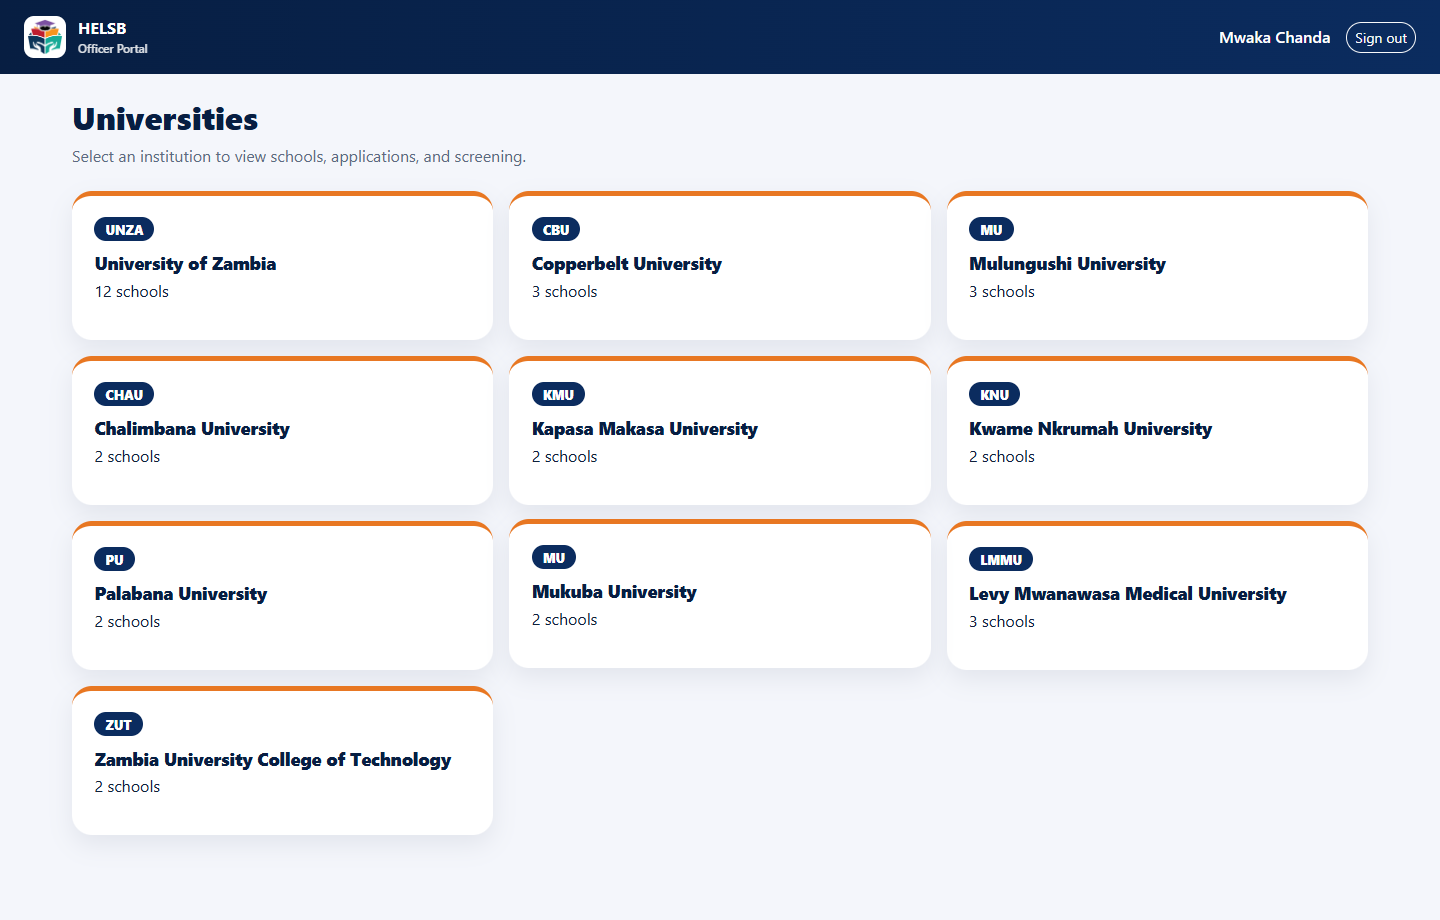
\includegraphics[width=\textwidth]{helsb-universities-desktop.png}
\caption{HELSB portal after sign-in: the university list}
\label{fig:helsb-universities}
\end{figure}

\begin{figure}[H]
\centering
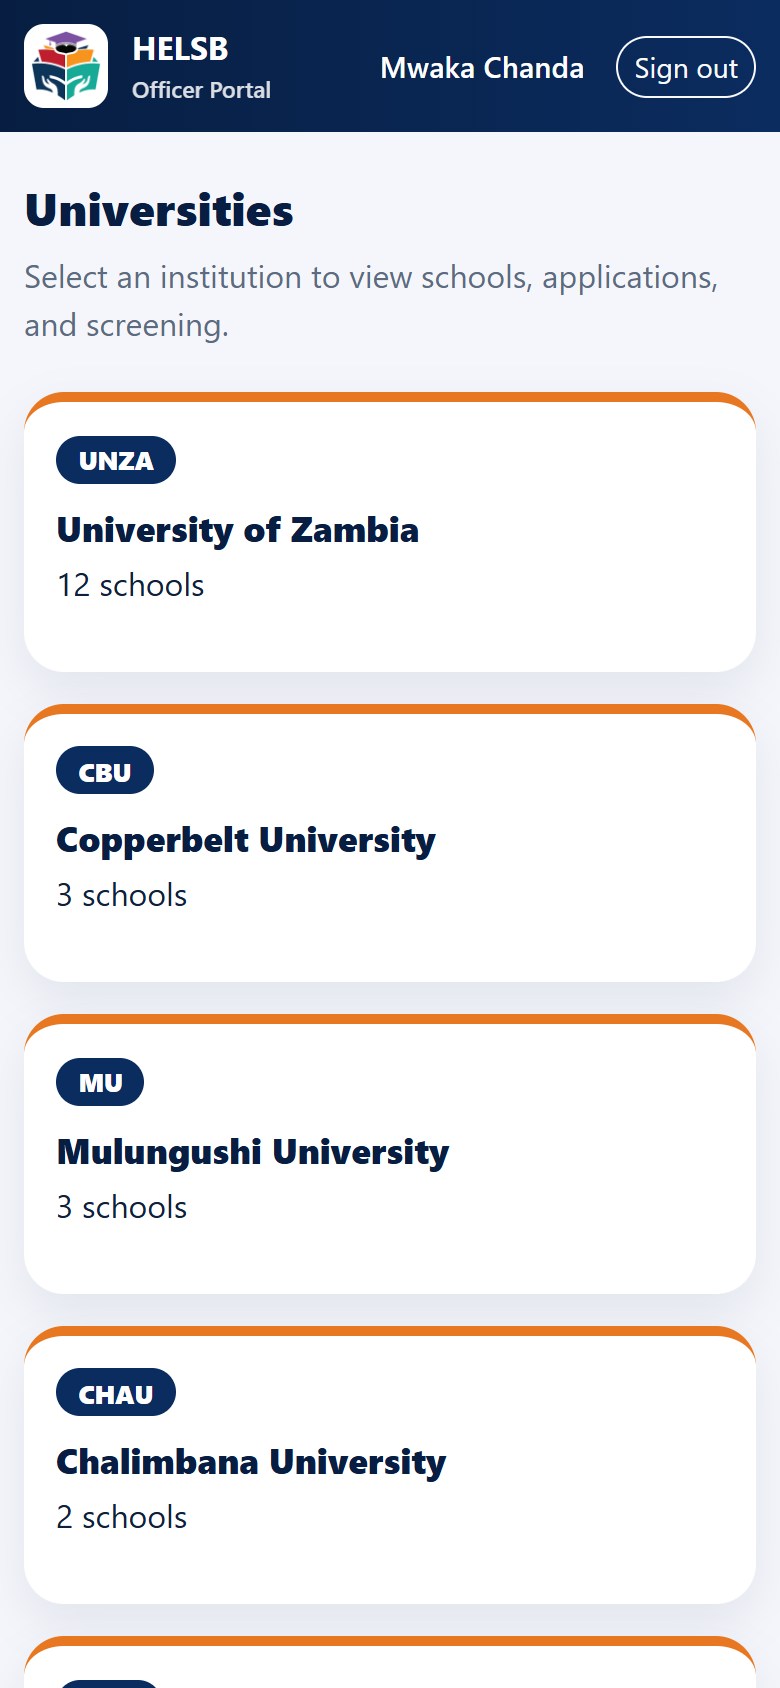
\includegraphics[width=0.48\textwidth]{helsb-universities-mobile.png}
\caption{The same university list at phone width}
\label{fig:helsb-mobile}
\end{figure}

\begin{figure}[H]
\centering
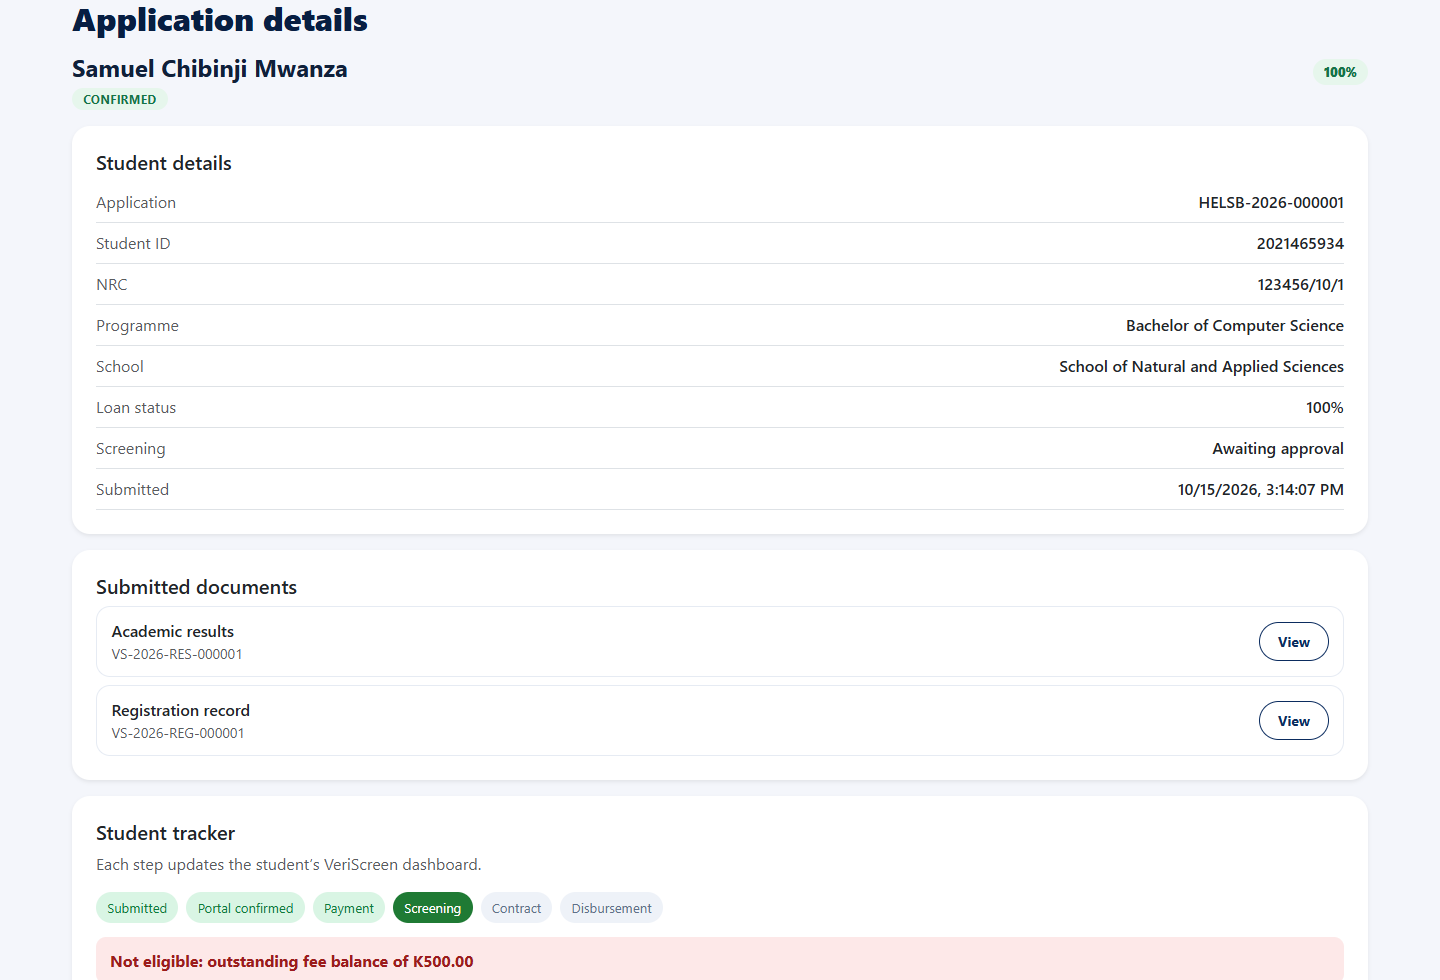
\includegraphics[width=\textwidth]{helsb-screening-desktop.png}
\caption{Officer view of Samuel Chibinji Mwanza at screening, with the same sentence shown on the student dashboard}
\label{fig:helsb-screening}
\end{figure}

\section{Algorithms / Models / Technical Design}
There is no machine-learning model. The technical core is the screening procedure in Table~\ref{tab:rules} and the pipeline in Table~\ref{tab:pipeline}.

\begin{table}[H]
\centering
\caption{HELSB pipeline}
\label{tab:pipeline}
\begin{tabular}{p{0.32\textwidth}p{0.55\textwidth}}
\toprule
Stage & Officer action that enters the next stage\\
\midrule
Submitted & Confirm in the portal\\
Portal confirmed & Record payment\\
Payment & Approve screening, which runs the explanation\\
Screening & Issue contract, only if the result is not ``Not eligible''\\
Contract & Mark disbursed\\
Disbursement & No further action\\
\bottomrule
\end{tabular}
\end{table}

The verification address is chosen when the document is generated. A public deployment address is used when one is configured. Otherwise the server uses a non-virtual local network address so that a phone on the same network can open the page. Virtual adapters such as a VPN interface are skipped because a phone cannot route to them.

\section{Chapter Summary}
The design splits the student and the officer, stores each side in its own database, and defines screening as an ordered list of record checks that produce one sentence.

\chapter{Implementation / Development}

\section{Introduction}
This chapter describes what was implemented in the completed local system.

\section{Development Environment}
The demonstration runs on a workstation with Node.js, MySQL, and two Vite development servers. The student API listens on all interfaces on port 8081. The officer API listens on port 8083. The student site is served at port 5173 and the officer site at port 5174. Each site proxies \texttt{/api} to its own API.

\section{System Components / Modules}
The student API implements sign-in, profile, registrations, fees, examinations, results, document listing, PDF download, the verification page, HELSB submission, and the internal endpoints for progress and screening. The officer API implements officer sign-in, the university and school catalogue, application retrieval, pipeline advance, and the call that requests a screening explanation. The student interface implements the dashboard tracker, documents, records, and the HELSB application view. The officer interface implements the university browser and the application tracker.

\section{Key Implementation Details}
PDF fee statements list the stored payments. The amount paid and the outstanding balance come from the fee rows. For Samuel the statement totals 14,000.00 billed, 13,500.00 paid, and a balance of 500.00. Results PDFs list the course code, grade, and a header containing the student name, computer number, and gender. The confirmation of registration is a portrait form filled from the registration and course rows. It does not invent an NRC, a birth date, or a course that is not stored.

The verification route \texttt{/verify/\{documentId\}} returns HTML. A known code such as Samuel's results document \texttt{VS-0E2BAD55} produces a green page titled ``Document verified''. An unknown code produces a red page stating that the code is not on an issued document. The JSON route \texttt{/api/verify/\{documentId\}} returns the same facts for a program client.

When the officer advances into screening, the officer service calls \texttt{/api/v1/internal/screen}. The student service applies Table~\ref{tab:rules} and returns the sentence. Both sides store it. The student dashboard polls the application and renders the sentence under the tracker.

\section{Integration}
Integration between the portals is the internal HTTP notification. The officer service sends the student computer number, the new stage, the application number, and, at screening, the explanation. The student service checks the internal key before it updates the student's application row. If the student has no row yet, one is created at the reported stage.

The university simulator is not called on every page view in the completed Node build. The demonstration record was loaded into \texttt{veriscreen\_db}. Document generation and screening both read that database, so the PDF and the sentence cannot diverge from each other by reading two different copies at the same moment.

\section{Challenges and Solutions}
The first hosting path depended on Java and PostgreSQL, which ordinary shared hosting does not provide. The APIs were rewritten in Node.js with MySQL, while PostgreSQL remains available when a hosted database URL is set.

QR codes originally preferred the first network address, which on the development machine was a Cloudflare WARP adapter. A phone on Wi-Fi could not open that address. Address selection now skips virtual adapters and uses the local network address, which on the test machine was \texttt{10.31.110.236}. An already downloaded PDF keeps the old code until the student downloads the document again.

An expired officer token left the officer name on screen and showed ``unable to load universities'', which looked like a stopped server. The officer client now clears the session when the API returns an authentication failure and returns the officer to the sign-in page.

A narrow PDF column clipped long names. The confirmation layout was widened and set in a fixed-width face so that the stored name and school could be printed in full.

\section{Individual Contribution (group projects)}
The repository is one group product. Appendix~A states the joint contribution of Samuel Chibinji Mwanza and Nosiku Mukuka. This chapter does not assign a private subsystem to either student beyond that appendix.

\section{Chapter Summary}
The implementation delivers two web portals, two APIs, two MySQL databases, PDF issue, phone verification, a six-stage tracker, and a rule-based screening sentence computed from the student record.

\chapter{Testing, Results and Evaluation}

\section{Introduction}
Testing checked the behaviours named in the objectives. The cases below were executed against the running local system.

\section{Testing Strategy}
System tests were used. Each case had a known student or officer, a single action, and an expected sentence or page. Unit tests of every function were not the measure of success, because the objectives are end-to-end. Regression checks consisted of repeating sign-in, document verification, and screening after the server was restarted.

\section{Test Cases and Results}
\begin{table}[H]
\centering
\caption{Representative system tests}
\label{tab:tests}
\begin{tabular}{p{0.10\textwidth}p{0.34\textwidth}p{0.32\textwidth}p{0.10\textwidth}}
\toprule
ID & Test case & Expected result & Status\\
\midrule
TC-01 & Sign in as 2021465934 & Dashboard opens for Samuel Chibinji Mwanza & Pass\\
TC-02 & Sign in with a wrong password & Sign-in is refused & Pass\\
TC-03 & Download Samuel's fee statement & Paid 13,500.00 and balance 500.00 & Pass\\
TC-04 & Open Samuel's results document & Name, computer number, and gender are present & Pass\\
TC-05 & Open \texttt{/verify/VS-0E2BAD55} & Green ``Document verified'' page & Pass\\
TC-06 & Open an unknown verification code & Red not-verified page & Pass\\
TC-07 & Officer sign-in and university list & Ten universities are returned & Pass\\
TC-08 & Advance Samuel to screening & ``Not eligible: outstanding fee balance of K500.00'' & Pass\\
TC-09 & Advance Nosiku to screening & Approved sentence, fees cleared & Pass\\
TC-10 & Advance Grace Banda to screening & Not eligible, balance K2,500.00 & Pass\\
TC-11 & Advance Peter Zulu to screening & Not eligible, balance K800.00 & Pass\\
TC-12 & Try to pass a ``Not eligible'' case & Pipeline stays on screening & Pass\\
TC-13 & Continue an approved case & Contract, then disbursement & Pass\\
TC-14 & Read the student application after TC-08 & Same stage and same sentence & Pass\\
\bottomrule
\end{tabular}
\end{table}

Nosiku's approved sentence is: ``Approved: good academic standing, fees cleared, registration confirmed.''

\section{Experimental Results / Performance Results (where applicable)}
No timing benchmark or load test was run. The relevant quantitative results are the record values that the sentences cite. Samuel's latest outstanding balance is K500.00. Grace Banda's is K2,500.00. Peter Zulu's is K800.00. Nosiku's latest outstanding balance is zero, her registration is confirmed, and her published grades support a GPA of at least 2.00, so the final rule applies.

\section{User Evaluation (where applicable)}
A formal user study was not conducted. Evaluation was by direct use of the student site and the officer site on the local machine, including the verification page on the Wi-Fi address of the student API.

\section{Analysis of Results}
The tests show that the document and the screening sentence are both functions of the stored record. Samuel is not described as fee-cleared, because his latest balance is K500.00. Nosiku is approved because the failing conditions do not apply. The student copy matches the officer copy after the internal notification. The failure mode that remains is environmental: a phone cannot open the verification page if it is on a different network or if the host firewall blocks port 8081.

\section{Objective-by-Objective Evaluation}
\begin{enumerate}
    \item The student portal signs in the seeded students and shows registration, fees, examinations, and results. Objective 1 was met for the demonstration data.
    \item PDF fee statements, results, and confirmation forms are generated from those rows. Objective 2 was met.
    \item A known code returns ``Document verified'' and an unknown code does not. Objective 3 was met on the computer and on the Wi-Fi address. A physical phone still depends on network reachability and the firewall.
    \item The officer portal lists institutions and advances the six-stage pipeline, and the student dashboard follows. Objective 4 was met.
    \item Screening produced the K500.00, K2,500.00, K800.00, and approved sentences from the records of the four students. Objective 5 was met.
\end{enumerate}

\section{Individual Results (group projects)}
The tests exercise the shared system. They are not split into personal scores. Appendix~A records that the result is a group deliverable.

\section{Chapter Summary}
The fourteen system tests passed. Each screening sentence matched the fee and academic rules, and the student view showed the officer's stage and explanation.

\chapter{Discussion}

\section{Introduction}
This chapter interprets the test results against the problem and the literature.

\section{Interpretation of Findings}
The project shows that a modest issuing service is enough to replace a screenshot for the demonstration. The verifier does not need an account. The code is either in the issued-document table or it is not. The project also shows that a loan status becomes clearer when the failing fact is written into the status. ``Not eligible'' alone would have hidden whether the cause was fees, registration, examinations, or grades. The K500.00 sentence can be checked against the fee statement for the same student.

\section{Comparison with Existing Work}
Compared with a portal screenshot, VeriScreen adds a server-side check and a stable document identifier. Compared with a digitally signed PDF, it is weaker against editing of the page around an intact QR code, and it is simpler to scan. Compared with a loan file that stores only a percentage, the officer portal stores the explanation that the rules produced. The system does not claim to implement a government production workflow.

\section{Contributions of the Project}
The practical contribution is a working pair of portals that a marker can sign in to and walk from a student record to a scanned page and then to an explained screening result. The technical contribution is the separation of the two databases with a narrow internal bridge, and the ordered screening rules that make the sentence deterministic.

\section{Limitations and Implications}
Because the rules are project rules, a different outstanding-balance threshold or a different GPA cut-off would change who is approved. Because the phone check only looks up the code, a forged page that still shows a genuine code would still verify. A production version would need signed document bytes, expiring codes, and a firewall and address story that does not depend on a developer's Wi-Fi. Simulated data mean that the tests do not measure accuracy against live UNZA records.

\section{Chapter Summary}
The findings support the aim inside the stated limits. Documents can be checked, and screening can be explained. The findings do not support a claim of legal equivalence to a university-signed transcript or an official HELSB decision.

\chapter{Conclusion and Recommendations}

\section{Introduction}
This chapter closes the report by returning to the aim and the five objectives.

\section{Summary of the Project}
VeriScreen and the HELSB officer portal were designed and implemented as a group project by Samuel Chibinji Mwanza and Nosiku Mukuka. Students sign in, read a simulated university record, and download PDFs. A QR code asks the issuing server whether the document exists. Officers move an application along a six-stage pipeline. Screening writes one sentence from fees, registration, examinations, and grades, and the student sees that sentence.

\section{Conclusions}
A separate issuer can make an academic PDF checkable on a phone without giving the verifier a university password. A separate officer portal can share pipeline state with that issuer through one internal call. Explainable screening is achievable when the rules are ordered and when each rule names the record it used. The demonstration data are sufficient to show both an approval and several fee-based refusals.

\section{Achievement of Objectives}
All five objectives were achieved for the local demonstration, with the reservation that phone scanning still requires a reachable address and an open port. The aim, a working web system that issues verifiable documents and explains screening, was met.

\section{Recommendations}
The development password should be removed before any public deployment. The verification port should be allowed through the host firewall by an administrator when a phone demonstration is required. Students should download documents again after the verification address changes, because an old PDF keeps its original code. The screening threshold should be confirmed with HELSB before anyone treats the sentence as an official eligibility decision.

\section{Future Work}
Future work should verify the PDF bytes rather than only the code, expire or revoke codes, connect to a real student information system under an agreement with the university, and replace the project screening rules with the Board's published rules if those rules are made available. A short usability study with students and officers would complement the system tests in Table~\ref{tab:tests}.

\clearpage
\chapter*{REFERENCES}
\addcontentsline{toc}{chapter}{References}

\begin{enumerate}
    \item Higher Education Loans and Scholarships Board. Official site. \url{https://www.helsb.gov.zm}.
    \item ISO/IEC 18004:2015. \textit{Information technology --- Automatic identification and data capture techniques --- QR Code bar code symbology specification}. International Organization for Standardization.
    \item Jones, M., Bradley, J., and Sakimura, N. (2015). \textit{JSON Web Token (JWT)}. RFC 7519. Internet Engineering Task Force. \url{https://www.rfc-editor.org/rfc/rfc7519}.
    \item Fielding, R. T. (2000). \textit{Architectural Styles and the Design of Network-based Software Architectures}. Doctoral dissertation, University of California, Irvine.
    \item Oracle Corporation. \textit{MySQL 8.0 Reference Manual}. \url{https://dev.mysql.com/doc/refman/8.0/en/}.
    \item Meta Open Source. \textit{React documentation}. \url{https://react.dev}.
    \item OpenJS Foundation. \textit{Express web framework for Node.js}. \url{https://expressjs.com}.
    \item OWASP Foundation. \textit{Authentication Cheat Sheet}. \url{https://cheatsheetseries.owasp.org/cheatsheets/Authentication_Cheat_Sheet.html}.
\end{enumerate}

\appendix

\chapter{Individual Contribution Statement (Group Projects)}

\section*{Purpose of this Statement}
This appendix is the group contribution statement for Samuel Chibinji Mwanza and Nosiku Mukuka. The system described in the report is a single product in one repository. The statement does not invent a private module split that was not recorded during development. Both students are responsible for the delivered student portal, officer portal, document service, and screening behaviour. A finer percentage split should be completed with the supervisor before binding if the department requires personal weights.

\section{Project and Group Information}

\begin{table}[H]
\centering
\begin{tabular}{p{0.35\textwidth}p{0.55\textwidth}}
\toprule
\textbf{Item} & \textbf{Details} \\
\midrule
Project title & VeriScreen: A Web-Based System for Academic Document Verification and HELSB Loan Screening \\
Students & Samuel Chibinji Mwanza (2021465934); Nosiku Mukuka (2022030346) \\
Supervisor & Mrs.\ Monde Monica Kalumbilo Kabemba \\
Group size & 2 \\
Group members & Samuel Chibinji Mwanza, 2021465934; Nosiku Mukuka, 2022030346 \\
\bottomrule
\end{tabular}
\end{table}

\section{Overall Group Project}
The group built VeriScreen, a student web portal that presents a simulated university record and issues PDF documents with QR verification, and a separate HELSB officer portal that advances a loan application and explains screening in plain language. The two portals exchange pipeline state through an internal API. The demonstration includes an approved student and students who are not eligible because of an outstanding fee balance.

\section{Individual Role and Responsibilities}
Both members worked on the shared system. The table records the areas of the product rather than a private assignment that the repository does not encode.

\begin{table}[H]
\centering
\begin{tabular}{p{0.08\textwidth}p{0.35\textwidth}p{0.42\textwidth}}
\toprule
\textbf{No.} & \textbf{Area of responsibility} & \textbf{Description} \\
\midrule
1 & Student portal & Sign-in, dashboard, records, documents, and the student tracker \\
2 & Document service & PDF layouts, QR address, and the verification page \\
3 & Officer portal & Universities, schools, applications, and the officer tracker \\
4 & Screening & Rules, stored explanation, and the stop on ``Not eligible'' \\
\bottomrule
\end{tabular}
\end{table}

\section{Detailed Individual Contribution}
The contribution of the group, undertaken by Samuel Chibinji Mwanza and Nosiku Mukuka, covers requirements for the student and officer workflows, the literature framing in this report, the analysis and design in Chapter~4, the Node.js and React implementation, the MySQL schema and seed data, the PDF and QR integration, the pipeline notification, the screening rules, the system tests in Chapter~6, and this written report. Work that originated in an earlier Java and PostgreSQL design in the same repository was retained where it still described the domain, and was replaced where the completed demonstration required Node.js and MySQL.

\section{Individual Deliverables}

\begin{table}[H]
\centering
\begin{tabular}{p{0.08\textwidth}p{0.35\textwidth}p{0.42\textwidth}}
\toprule
\textbf{No.} & \textbf{Deliverable} & \textbf{Group contribution} \\
\midrule
1 & Student web portal & Sign-in, records, documents, dashboard tracker \\
2 & HELSB officer portal & Catalogue, application detail, pipeline actions \\
3 & Issued PDF documents & Fee statement, results, confirmation, verification code \\
4 & Screening explanation & Plain-language result shown to officer and student \\
5 & This report & Account of the completed system \\
\bottomrule
\end{tabular}
\end{table}

\section{Contribution to the Main System or Research Output}
The final output is the integrated demonstration: a student can obtain a document, a verifier can scan it, and an officer can screen the same student and produce a sentence the student can read. No component is described here as the sole work of one member.

\section{Individual Implementation and Technical Work}
The technical work includes the Express services under \texttt{veriscreen/server} and \texttt{helsb-portal/server}, the React sources under \texttt{veriscreen/frontend} and \texttt{helsb-portal/frontend}, the MySQL setup in the server database modules, PDF generation, the \texttt{/verify} page, and the screening function. Configuration for a hosted PostgreSQL database is included so that the same services can leave the local MySQL installation.

\section{Individual Testing and Evaluation Contribution}
The group executed the cases in Table~\ref{tab:tests}, including Samuel's K500.00 result, Nosiku's approval, Grace Banda's K2,500.00 result, Peter Zulu's K800.00 result, and the verification page for \texttt{VS-0E2BAD55}.

\section{Collaboration with Other Group Members}
The student portal depends on the officer portal for stage changes, and the officer portal depends on the student API for the screening sentence. Those dependencies are inside the group product. No external student supplied a hidden module.

\section{Contribution Summary}
\begin{enumerate}
    \item Work completed by the group: the portals, APIs, documents, tracker, screening, tests, and this report.
    \item Work completed jointly: the whole demonstration path from sign-in to disbursement.
    \item Work completed by others and used here: published platform documentation cited in the references, and the department report template that structures this document. Seeded academic figures are simulated project data, not a live university extract.
\end{enumerate}

\section{Estimated Contribution}
A numeric split between the two students was not logged as a separate measurement. The table therefore records the work as collaborative. The students should replace the dashes with agreed percentages before submission if the department requires them.

\begin{table}[H]
\centering
\begin{tabular}{p{0.45\textwidth}p{0.20\textwidth}p{0.20\textwidth}}
\toprule
\textbf{Project activity} & \textbf{Individual} & \textbf{Collaborative} \\
\midrule
Problem analysis & --- & Group \\
Literature review & --- & Group \\
Requirements analysis & --- & Group \\
System design & --- & Group \\
Implementation & --- & Group \\
Testing and evaluation & --- & Group \\
Documentation & --- & Group \\
\bottomrule
\end{tabular}
\end{table}

\noindent
\textit{Note: The department template asks for approximate percentages. They are intentionally not invented here. They are not required to total 100 percent across rows once the students enter them.}

\section{Statement of Authorship and Contribution}
We confirm that this statement describes the joint system truthfully. We have not knowingly assigned one member's work to the other, because the delivered system is recorded as shared work.

\vspace{1cm}
\noindent\textbf{Student Name:} Samuel Chibinji Mwanza

\vspace{0.5cm}
\noindent\textbf{Computer Number:} 2021465934

\vspace{0.5cm}
\noindent\textbf{Signature:} \hrulefill

\vspace{0.5cm}
\noindent\textbf{Date:} \hrulefill

\vspace{1cm}
\noindent\textbf{Student Name:} Nosiku Mukuka

\vspace{0.5cm}
\noindent\textbf{Computer Number:} 2022030346

\vspace{0.5cm}
\noindent\textbf{Signature:} \hrulefill

\vspace{0.5cm}
\noindent\textbf{Date:} \hrulefill

\newpage
\section{Supervisor Verification}
I confirm that, to the best of my knowledge, the contribution described above is consistent with the students' participation in the group project.

\vspace{1cm}
\noindent\textbf{Supervisor Name:} Mrs.\ Monde Monica Kalumbilo Kabemba

\vspace{0.5cm}
\noindent\textbf{Signature:} \hrulefill

\vspace{0.5cm}
\noindent\textbf{Date:} \hrulefill

\chapter{User Manual / Installation Guide}

\section*{What must be running}
Install Node.js and MySQL. Create the databases by starting each API once. The student API creates and seeds \texttt{veriscreen\_db}. The officer API creates and seeds \texttt{helsb\_db}. The local MySQL account used in development is \texttt{root} with the development password configured in each server environment file.

\section*{Start order}
\begin{enumerate}
    \item Start the student API in \texttt{veriscreen/server} with \texttt{node server.js}. It listens on port 8081.
    \item Start the officer API in \texttt{helsb-portal/server} with \texttt{node server.js}. It listens on port 8083.
    \item Start the student site in \texttt{veriscreen/frontend} with \texttt{npm run dev}. Open \url{http://localhost:5173/login}.
    \item Start the officer site in \texttt{helsb-portal/frontend} with \texttt{npm run dev}. Open \url{http://localhost:5174}.
\end{enumerate}

\section*{Demonstration accounts}
Every development password is \texttt{password123}.

\begin{table}[H]
\centering
\caption{Accounts for the demonstration}
\begin{tabular}{p{0.28\textwidth}p{0.28\textwidth}p{0.32\textwidth}}
\toprule
Person & Sign-in & What screening shows\\
\midrule
Samuel Chibinji Mwanza & 2021465934 & Not eligible, balance K500.00\\
Nosiku Mukuka & 2022030346 & Approved\\
Grace Banda & 2020123456 & Not eligible, balance K2,500.00\\
Peter Zulu & 2019876543 & Not eligible, balance K800.00\\
Mwaka Chanda & mwaka.chanda@helsb.zm & Officer\\
Chanda Phiri & chanda.phiri@helsb.zm & Officer\\
\bottomrule
\end{tabular}
\end{table}

\section*{Suggested walk-through}
Sign in as a student and open Records, Results, and Documents. Download a PDF again if the QR code must work on a phone, then scan it while the phone is on the same Wi-Fi. Sign in as an officer, open the University of Zambia, open the student's school, and advance the pipeline until screening. Leave the student dashboard open. It refreshes and shows the same sentence.

\section*{Troubleshooting}
If the officer page says that universities could not be loaded, sign in again. An old token is rejected. If a phone cannot open the verification page, confirm that the PDF was downloaded after the server restart, that the phone is on the same Wi-Fi, and that Windows Firewall allows inbound TCP on port 8081.

\chapter{Additional System Designs / Diagrams}
No separate diagram file is embedded in this report. The architecture is fully described by Table~\ref{tab:processes}, Table~\ref{tab:rules}, and Table~\ref{tab:pipeline}. Those tables are the design record for the completed build: two portals, two databases, one internal bridge, six pipeline stages, and six screening outcomes of which the last is approval.

\chapter{Additional Test Cases and Results}
The verification page for a known document states the document type, the student name, the computer number, and the code. Samuel's seeded documents include academic results \texttt{VS-0E2BAD55}, a fee statement \texttt{VS-1B14F7FB}, a confirmation of registration \texttt{VS-C952B77C}, and an examination slip \texttt{VS-C6B84BDF}. Opening any of those codes on the student API returns ``Document verified''. Samuel's results page was confirmed on \texttt{http://10.31.110.236:8081/verify/VS-0E2BAD55} during testing. That address belongs to the development machine and will differ on another network.

\chapter{Data Collection Instruments}
No questionnaire, interview guide, or participant consent form was used. The project did not collect data from human participants. The demonstration records were authored as seed data for the system.

\chapter{Additional Code / Configuration}
The complete source is in the project repository. The behaviour described in this report is concentrated in the following places.
\begin{itemize}
    \item \texttt{veriscreen/server/server.js} for sign-in, documents, verification, and screening.
    \item \texttt{veriscreen/server/pdf.js} for the PDF layouts.
    \item \texttt{veriscreen/server/db.js} for the student schema and seed.
    \item \texttt{helsb-portal/server/server.js} for the officer pipeline and the screening call.
    \item \texttt{helsb-portal/server/db.js} for officers and applications.
    \item \texttt{veriscreen/frontend} and \texttt{helsb-portal/frontend} for the two interfaces.
\end{itemize}
Environment files hold the database password and the token secret. They are not reproduced in this appendix.

\chapter{Other Supporting Material}
The department template supplied the chapter order, the declaration and approval pages, and the group-project appendix. The example references in that template, which concern crop yield and disease forecasting, were not cited because they are not sources for this system. The references in this report are the sources actually used to describe QR codes, tokens, REST, MySQL, React, Express, authentication practice, and HELSB.

\end{document}
